%\chapter{3HDM}
%

\newpage 

\chapter{3HDM Model}
\label{ch:3HDM}
%\section{Not used yet}

%We used previous work to narrow down the vast parameter space of these type of models offer, see \cite{Ferreira_2018,Ivanov_2012,Ivanov_2016,Aranda_2017}.
%
%Our conclusions are consistent with these studies, where it was found to have large regions of parameter space which conformed with experimental constraints in the flavour and scalar sectors.

%\section{Introduction}

Now having finished the analysis of a simple unitary extension, it is time to present a more complex model. 
%
The goal of this chapter will be to first introduce all the required theoretical background to the analysis of a three Higgs Doublet Model (3HDM), specifically a minimal BGL (Branco-Grimus-Lavoura) like 3HDM, such as presented in Ref.~\cite{Ludvig_Thesis}. 
% 
Then moving to present a phenomenological simulation similar as before, as to observe the state of the art in the 3HDM. 
%
This simulation used a newer version of the previously discussed mechanism with the addition of a flavour calculation package based on python3 entitled \texttt{flavio} \cite{straub2018flavio}. 

This 3HDM model is part of a larger family of multiple Higgs Doublet Models, or NHDMs, the first iteration of which was the Two Higgs Doublet Model (2HDM) model. 
% 
As mentioned before, one of the simplest ways to expand the SM is to add elements to its scalar sectors.
%
In these types of models, in parallel with the standard SM Higgs doublet some additional replicas of that same doublet are introduced. 
%
In the 3HDM these form a sort of family in the scalar sector in analogy to the fermion sector. 
%
This idea is far from original and was first discussed by Weinberg in, \cite{Weinberg1976}.

These additional Higgs are valid given they do not alter the tree-level electroweak $\rho$ parameter as long the condition that the sum of the doublet VEVs are equal to the value of the electroweak VEV in case of the SM {\color{blue} citation needed}. 
% 
Although this value can vary by 20\% { \color{blue} citation needed} there are many reasons as to impose this condition.
%
This is part of a wider \textit{alignment limit} condition that will be discussed further on. 
%
The basis for our BGL like treatment of a 3HDM will be the inclusion of a flavour symmetry, as to attempt to constrain the flavour observables. In particular the addition of a $\mathrm{U}(1) \times \mathrm{Z}_2$ symmetry.
% 
This symmetry constrains the terms that can appear in the flavour sector of the Lagrangian resulting in very specific structures (or textures) of the Yukawa couplings.
% 
We will show how this structure combined with the off diagonal terms of the CKM matrix lead to controlled values for FCNCs. 
%
% achieving a similar mechanism to that of the BGL 2HDM. 
%
Then showing that light scalars are still within the reach of future collider experiments in our model's framework while having FCNCs concurrent with observations and respecting many more theoretical and experimental bounds, such as in our previous analysis. 


\subsection{Context, the case of the BGL-2HDM}

The first model that attempted to perform a doublet based extension was the 2HDM proposed by T.D. Lee \cite{Lee1973}.  
%
His work was motivated by the search for a spontaneous breaking of the CP symmetry. 

A great deal of interest was invested in 2HDMs, given the possiblity for dark matter candidates, as well as providing a large particle spectrum, including charged and additional neutral scalars.
%
However, most 2HDM structures allow for the possibility of tree-level scalar mediated FCNCs. 
% 
An analysis of their origin led to disturbing conclusions, given that fermions now have their mass generated by several Yukawa matrices and their simultaneous diagonalisation was not always guaranteed. 
%
These tree-level FCNCs are, in most cases, in direct opposition to experimental results, as discussed in chapter~\ref{Chap:SM}, section~\ref{Chap_1_Sec_3}. 
%
In fact, consulting the literature, as in, \cite{Branco:1999fs}, we see that this forces the extra scalars in the 2HDM case to have masses above 1 TeV.
%
These heavy scalars are far from ideal, since there is no indication such heavy scalars exist nor do they provide us with interesting physics. 
%
There-for several mechanisms have been proposed to deal with suppress these tree-level FCNCs as to allow for richer physics. 
%
First, in, \cite{Ferreira_2011,Nebot_2015,ferreira2019strong}, it is proposed a framework in which we have the balancing of CP-odd and CP-even contribution to FCNCs, however, this requires some fine-tuning, making it very unappealing. 
% 
Another possibility is to assume alignment between different Yukawa matrices such that no FCNCs are present, see \cite{Pich_2009,Jung_2010,Jung_2011} for more information. 
%
Finally we could also use the approach presented in the BGL version of the 2HDM \cite{Branco_1996,LAVOURA1994}, here the authors impose a flavour-violating symmetry naturally keeping the FCNCs under control trough the CKM matrix. 
%
The phenomenology of the model has been studied quite thoroughly in previous works, see Refs. \cite{Botella_2014,Botella_2016}, and it remains a possible scenario for BSM physics.
%
Inspired by this BGL model our studies will try to reproduce a similar mechanism on a 3HDM Model. 


\section{The formulation of a BGL-like 3HDM} 

Challenging the 2HDM BGL paradigm can be motivated by some phenomenological comparison of the 3HDM to the 2HDM model besides the "naturalist" family argument.
%
For example, vacuum stability in the 2HDM model can only accommodate one instance of spontaneous CP or charge symmetry breaking \cite{Branco_2012,Ferreira_2004,Barroso_2007}. 
%
However in NHDMs, such as the 3HDM, charge breaking minima were found to be stable while at the same time coexisting with charge-preserving ones, for more information see, \cite{Barroso_2006}.   
%
Also, for the 2HDM a full list of all possible incorporations of symmetries consistent with $\mathrm{SU(2)}\times\mathrm{U(1)}$ has been achieved \cite{Ivanov_2008,Ivanov2007}, while for the 3HDM no work has thus far been completed, see, \cite{Ivanov_2012,Ivanov_2015}. 
%
Moreover generic unitarity constraints have been found for the 2HDM \cite{Ginzburg_2005} but not for 3HDMs. 
%
Not to mention these models provide a richer playground for experimental detection and testing than the 2HDM given its extended scalar sector. 

\subsection{Fields and the Additional \texorpdfstring{ $\mathrm{U(1)}\times\mathbb{Z}_2$}{} Symmetry}

In a sense this model is an extension of the SM as it still includes all the same fields with same charges under the $\mathcal{G}_{SM}$ as we saw in chapter~\ref{Chap:SM}. 
% 
Making the particle content of the model the same as the SM with the addition of new scalars. 
%
%Having the same gauge fields and the following fermion and scalar fields,
Consequently, we have,
%
\begin{equation}
\label{eq:3HDM_Fields}
\begin{gathered}
Q_{L_i} =  \begin{pmatrix}
u_{L_i}  \\
d_{L_i}
\end{pmatrix} \quad , \quad \Psi_{L_i} =  \begin{pmatrix}
\nu_{L_i}  \\
e_{L_i}
\end{pmatrix} \quad , \quad \\ 
u_{R_i} \quad , \quad d_{R_i} \quad , \quad e_{R_i} \quad i=\{1,2,3\} \quad ,  \\  
\phi_k = \begin{pmatrix}
W_k^\pm + i \, W_k^\mp \\ 
\frac{1}{\sqrt{2}}\left( v_k + h_k + i Z_k \right) 
\end{pmatrix}  \quad , \quad k=\{ 1,2,3\} \quad . 
\end{gathered} 
\end{equation}
%
where $Q_{L_i}$ , $\phi_k$ and $\Psi_{L_i}$ are $\mathrm{SU(2)_L}$ doublets while $u_{R_i}$, $d_{R_i}$, and $e_{R_i}$ are $\mathrm{SU(2)_L}$ singlets where the i and k generation stand for their respective generation indexes. 
%
However the new charges under $\mathrm{U(1)}\times\mathbb{Z}_2$ must be specified. 
%
They show themselves in the transformations that these fields undergo, 
%
\begin{equation}
\label{eq:3HDM_Transformations}
	\begin{split} 
	\mathrm{U(1)} : & \\
		& Q_{L_3} \rightarrow    e^{i \alpha} Q_{L_3}  \\  
		& u_{R_3} \rightarrow    e^{2 i \alpha} u_{R_3}  \\
		& \phi_1  \rightarrow    e^{i \alpha} \phi_1  \\   
		& \Psi_{L_1} \rightarrow e^{i \alpha} \Psi_{L_1} \\
		& \phi_3 \rightarrow     e^{i \alpha} \phi_3  \\ 
	\end{split} \quad \quad \quad  
	\begin{split}
		\mathbb{Z}_2 : & \\
		 	& Q_{L_3} \rightarrow -Q_{L_3} \\
		 	& u_{R_3} \rightarrow -u_{R_3} \\ 
		 	& \phi_1  \rightarrow -\phi_1 \\ 
		 	& \Psi_{L_1} \rightarrow - \Psi_{L_1} \\ 
		 	& \phi_3 \rightarrow -\phi_3
	\end{split} 
\end{equation} 
%
All remaining fields not shown in Eq. \ref{eq:3HDM_Transformations} remain unchanged under transformations of the $\mathrm{U(1)}\times\mathbb{Z}_2$ global symmetry (one scalar field and two fermion generations).  
%
This symmetry will have to be softly broken as to avoid the appearance of a massless Goldstone state.

Note there is no right handed neutrino fields in this model making it so that no neutrino mass terms appear.

\subsection{Introducing the Scalar Sector}

Let us then start our proper introduction to the workings of the model by presenting the scalar sector where the new spin-0 $\mathrm{SU(2)}$ doublets, $\phi_i$, $i=\{1,2,3\}$ reside.
%
\begin{comment}
The scalar doublets are made to transform under the imposed $\mathrm{U(1)}\times \mathbb{Z}_2$ symmetries as, 
%
\begin{equation}
\begin{split}
\mathrm{U(1)} & : \phi_1 \rightarrow \phi_1 e^{i \alpha} \quad ,
            \quad \phi_3 \rightarrow \phi_3 e^{i \alpha}  \\
\mathbb{Z}_2  & : \phi_1 \rightarrow -\phi_1 \ \ \quad , 
            \quad \phi_2 \rightarrow \phi_2  \quad , 
            \quad \phi_3 \rightarrow \phi_3 \quad .
\end{split}
\end{equation}
\end{comment}
Note the scalar potential is $\mathcal{CP}$-invariant, this means, 
\begin{equation}
\phi_1 = \phi_1^{\**} \quad , \quad \phi_2 = \phi_2^{\**} \quad , \quad 
\phi_3 = \phi_3^{\**} 
\end{equation}
 { \color{red} Não falta um sinal de menos no $\phi_{1,3}$ Eu disse que o outro não se transforma sobre Z2 mas como isto é CP trans. não devia de ter? Ask morais } 

The generic scalar potential that follows all these transformations is extensively written in, 
\begin{equation}
\label{eq:3HDM_Scalar_Pot}
\begin{split}
V(\phi_i) = & 
- \mu_1^2 \left( \phi^{\dagger}_1 \phi_1 \right) 
- \mu_2^2 \left( \phi^{\dagger}_2 \phi_2 \right)  
- \mu_3^2 \left( \phi^{\dagger}_3 \phi_3 \right) \\ 
& \left[ - \mu_{12}^2 \left( \phi^{\dagger}_1 \phi_2  \right) 
  - \mu_{23}^2 \left( \phi^{\dagger}_2 \phi_3  \right)  
  - \mu_{13}^2 \left( \phi^{\dagger}_1 \phi_3  \right) + h.c. \right]  \\
& + \lambda_1 \left( \phi^{\dagger}_1 \phi_1 \right) 
  + \lambda_2 \left( \phi^{\dagger}_2 \phi_2 \right)  
  + \lambda_3 \left( \phi^{\dagger}_3 \phi_3 \right) \\  
& + \lambda_4 \left( \phi^{\dagger}_1 \phi_1 \right)  \left( \phi^{\dagger}_2 \phi_2 \right) 
  + \lambda_5 \left( \phi^{\dagger}_1 \phi_1 \right)  \left( \phi^{\dagger}_3 \phi_3 \right)  
  + \lambda_6 \left( \phi^{\dagger}_2 \phi_2 \right)  \left( \phi^{\dagger}_3 \phi_3 \right)  \\ 
& + \lambda_7 \left( \phi^{\dagger}_1 \phi_2 \right)  \left( \phi^{\dagger}_1 \phi_2 \right)  
  + \lambda_8 \left( \phi^{\dagger}_1 \phi_3 \right)  \left( \phi^{\dagger}_3 \phi_1 \right)   
  + \lambda_9 \left( \phi^{\dagger}_2 \phi_3 \right)  \left( \phi^{\dagger}_3 \phi_2 \right)  \\
& + \lambda_{10} \Bigg\{ \left( \phi^{\dagger}_1 \phi_3 \right)^2 + \text{H.c.} \Bigg\}   
\end{split} 
\end{equation}
%
{ \color{red} Este potencial tem de ser visto com cuidado. Primeiro, os termos com $\lambda_{1,2,3}$ são iguais aos termos com $\mu^2_{1,2,3}$ mas com o simal trocado. Segundo, porque que é que o $\lambda_{10}$ é o único com Hermıitico conjugado? Não estamos a fazer double counting com isto} 

Due to the $\mathcal{CP}$ symmetry imposed on this potential all parameters, $(\lambda_i,i=\{1,...,10\})$, here are real.
%
The parameter $\mu_{23}$, is necessarily added as to impede the formation of a massless axion. 
%
However the most generic version of this soft breaking is given by the second line. {\color{red} Porque?
Todos os termos da segunda linha são genéricos de um potential 3HDM. Não?} 
%
Of these note that the $\mu^2_{23}$ term is the only one that respect the $\mathbb{Z}_2$ symmetry. 
%
A study of these part of the flavor symmetry, has been included in the first analysis of Ref.~\ref{Ian_Thesis}.
%
After the process of SBB, all Higgs doublets take a VEV shape similar to that of the SM Higgs, written as, 
%
\begin{equation}
\phi_k = 
\begin{pmatrix}
W_k^\pm + i \, W_k^\mp \\ 
\frac{1}{\sqrt{2}}\left( v_k + h_k + i Z_k \right)
\end{pmatrix}  \rightarrow \langle \phi_k \rangle = \begin{pmatrix}
0 \\ 
\frac{v_k}{\sqrt{2}}
\end{pmatrix} \quad , \quad k=\{ 1,2,3\} 
\label{eq:3HDM_Higgs_Field_VEV}
\end{equation} 
%
Here we see the charged portion of the field, $W_k^\pm$, the CP-odd portion, $Z_k$, and finally the CP-even, $h_k$. 
%
Note that after SBB there will still remain 3 massless states (goldstone bosons) that will be later absorved into the gauge bosons $W$ and $Z$. This allows for them to be removed from the scalar spectrum.

Recall that, for the given scalar potential $V$ as seen in Eq \ref{eq:3HDM_Scalar_Pot} to have a stable vacuum it needs to satisfy \textit{boundness from below} conditions. 
%
As before this will ensure that there is indeed an absolute minimum of energy. 
%
To solve these one must write the derivates of the potential with respect to the fields and then observe their values once the process of SBB occurs, this process yields the following equations,
%
\begin{equation}
\label{eq:3HDM_tadpoles}
\begin{split}
\frac{\partial V}{\partial \phi_1} = & \frac{1}{2} v_1 \left( \left( 2 \lambda_{10} + \lambda_5 + \lambda_8 \right) v_3 + 2 \left( \lambda_1 v_1 + \mu_1^2 \right) + \left( \lambda_4 + \lambda_7 \right)  \right)  \\ 
\frac{\partial V}{\partial \phi_2} = & \frac{1}{2} v_2 \left( 2\left( \lambda_2 v_2^2 + \mu_2^2 \right) + \left( \lambda_4 + \lambda_7 \right) v_1^2 + \left( \lambda_9 + \lambda_6 \right)v_3^2 \right) + \mu_{23} v_3 \\
\frac{\partial V}{\partial \phi_3} = & \frac{1}{2} \left( \left( 2 \lambda_{10} + \lambda_5 + \lambda_8  \right) v_1^2  + 2 \mu_3^2 + \left( \lambda_6 + \lambda_9 \right) v_2^2 \right) v_3 + \lambda_3 v_3^3 + \mu_{23}^2 v_2 \\
\end{split} 
\end{equation}
%
By requiring that the derivatives of the potential vanish for some value of the CP-even fields $\phi_i$ , one arrives at the so-called tadpole equations of the model.
%
And trough the tadpole equations in Eq. \ref{eq:3HDM_tadpoles}, we could express the quadratic terms $\mu_1$, $\mu_2$ and $\mu_3$ as follows, 
%
\begin{equation}
\label{eq:3HDM_Param_1}
\begin{split}
\mu_1^2 & = \lambda_1 v_1^2 + \frac{1}{2} \left( \lambda_4 + \lambda_7 \right) v^2_2 + \frac{1}{2} \left( \lambda_5 + \lambda_8 + 2 \lambda_{10} \right) v_2^2  \\ 
\mu_2^2 & = \lambda_2 v_2^2 + \frac{1}{2} \left( \lambda_4 + \lambda_7 \right) v_1^2 + \frac{1}{2} \left( \lambda_6 + \lambda_9 \right) v_3^2 +\frac{v_3}{v_2} \mu^2_{23}  \\
\mu_3^2 & = \lambda_3 v^2_3  + \frac{1}{2}\left( \lambda_6 + \lambda_9 \right) v^2_2 + \frac{1}{2} \left( \lambda_5 + \lambda_8 + 2 \lambda_{10} \right)v_1^2 + \frac{v_2}{v_3} \mu_{23}^2 
\end{split}  
\end{equation}

\subsubsection{The Alignment Limit}

Let us first consider the gauge portion of the 3HDM Lagrangian. After the Higgs Doublets shift to their VEVs we have the following mass terms, 
%
\begin{equation}
\mathcal{L}_{\text{gauge}} \supset \frac{1}{4} \left( v_1^2 + v_2^2  + v_3^2 \right) g^2 W^+_\mu W^{-\,\mu} + \frac{1}{8} \left(  v_1^2 + v_2^2  + v_3^2  \right) \left( g^{\prime \, 2} + g^2 \right) Z_\mu Z^\mu  
\end{equation}
where we can clearly see that to reproduce the correct gauge boson masses we must ensure that, 
\begin{equation}
\label{eq:VEV_Condition}
\sum_{k=1}^3 v_k^2 \approx 246^2 \text{GeV} \quad . 
\end{equation}
This is a very important condition as it will reflect what range of values are available for our Higgs Doublets to take. Recall that the couplings to the Higgs bosons have been precisely measured making this the only way to achieve the correct gauge spectrum. 
%
It is convenient for us to perform the following parametrization,
%
\begin{equation}
v_1 = v \cos(\psi_1) \cos(\psi_2) \quad , \quad v_2 = v \sin(\psi_1) \cos(\psi_2) \quad , \quad v_3 = v \sin(\psi_2)
\end{equation}
where now the VEVs are written as a combination of a magnitude $v=\sqrt{v_1^2 + v_2^2 + v_3^2 }$ and two mixing angles $\psi_1$ and $\psi_2$. 

Through this parametrization we can write the orthogonal mixing matrix, 
\begin{equation}
\label{eq:3HDM_Orthg}
\mathcal{O} = 
\begin{pmatrix}
\cos(\psi_1) \cos(\psi_2) & \cos(\psi_2) \sin(\psi_1) & \sin(\psi_2) \\ 
- \sin(\psi_1) & \cos(\psi_1) & 0 \\ 
- \cos(\psi_1) \sin(\psi_2) & \sin(\psi_1) \sin(\psi_2) & \cos(\psi_2)
\end{pmatrix}
\end{equation}
%
This matrix is going to form a fundamental part of the diagonalization of massive scalar states. 
% 
This matrix will be responsible for giving us a intermediate basis, between the gauge and mass basis, that we will call the Higgs basis. { \color{red} parei de reler aqui } 
%
It is also going to form a crucial part of our numerical and theoretical studies, as it's going to be a key component of the the \textit{inversion process}. What we mean by this inversion process is simply to write all the terms of the Lagrangian in terms of physical parameters, these are mixing angles and masses. 

Asides from ensure the proper Gauge boson masses we must also account for the proper Gauge-Higgs interactions. We observe Lagrangian terms of the form, 
\begin{equation}
\frac{g^2 v}{2} W^+_\mu W^{\mu \, -} \left( \frac{1}{v} \sum_{k=1}^3 h_k v_k \right) 
\end{equation}
We clearly see this to be CP-even Higgs states interacting with the $W^\pm$ bosons, so apriori we must ensure that this represents a physical state relating to the SM Higgs Boson as, 
\begin{equation}
h_1 = \left( \frac{1}{v} \sum_{k=1}^3 h_k v_k \right) 
\end{equation}
Otherwise different tree-level couplings to the gauge bosons would show themselves. This can be explicitly desmostrated and is shown in Ref.~\cite{das2015implications} 

This procedure is also called Higgs alignment limit. Where we force a eigenstate of the Gauge base to serve as the observed Higgs Boson, leading to a complete superposition of both physical and gauge eigenstates. For a more detailed description of the process see Ref. \cite{Ian_Thesis}.  
%
Note however, although we use a "perfect alignment" there is room for some of the Higgs boson to be a mixture of other scalar states of this kind (about $\mathcal{O}(10\%)$, as discussed in \ref{Aad_2020}. 

\subsection{The CP-odd portion of the scalar sector}

We can now turn our attention to the physical scalar spectrum of the model. 
%
This potential is explicitly CP invariant given all parameters are real (VEVs, couplings and quadratic masses). In fact in this model we expect to find no more sources of CP-violation than in the SM.

\subsubsection{Pseudoscalar Eigenstates}

The CP-odd portion of the scalar sector (related to the $z_k$ degrees of freedom) contains quadratic terms after the process of SBB. 
%
These are easily extracted from the scalar potential in the form, 
%
% of quadratic terms of the $z$ fields once SBB takes place, seen as, 
\begin{equation}
V_{\text{shifted}} \supset \left( \begin{array}{ccc} z_1 & z_2 & z_3 \end{array} \right) \frac{M_P^2}{2} \left( \begin{array}{c} z_1 \\ z_2 \\ z_3 \end{array} \right)  
\end{equation}
%
where $M_P^2$ is the $3\times3$ pseudoscalar mass matrix in a non diagonal form, i.e. in a unphysical basis. 
%
It can however be expressed in a block diagonalized trough the rotation matrix we introduced in Eq. \ref{eq:3HDM_Orthg}, as,
%
\begin{equation}
B^2_P = \mathcal{O} M_P^2 \mathcal{O}^T = \left( \begin{array}{ccc}
0 & 0 & 0 \\ 
0 & \left( B^2_P \right)_{22} &  \left( B^2_P \right)_{23} \\
0 & \left( B^2_P \right)_{32} &  \left( B^2_P \right)_{33}
\end{array} \right) 
\end{equation}
%
The line and column of zeroes in this matrix tells us that it has a zero eigenvalue. This eigenstate will provide a Goldstone, this is clearly the Goldstone that will become the longitudinal polarization of the $Z$. 
%
%which of course, is the neutral Goldstone boson that the $Z$ gauge boson will later-on "latch-on" to.
%
The remaining elements of the $B^2_P$ matrix are given by,
\begin{equation}
\begin{split}
\left( B^2_P \right)_{22} = &  \frac{ 
v_3 \left( -2 v^3_2 v_3 \lambda_10 +  v_1^2 \mu_{23}^2 \right) } 
{v_2 \left( v_1^2 + v_2^2 \right)  }  
\\
\\ 
\left( B^2_P \right)_{32} = & \left( B^2_P \right)_{23} = \frac{v_1 v \left( 2 v_2 v_3 \lambda_{10} + \mu_{23}^2 \right) }{v_2^2 + v_1^2} \\
\\
\left( B^2_P \right)_{33} = & \frac{v^2 \left( 2 v_1^2 v_3 \lambda_{10} - v_2 \mu_{23}^2 \right) }{\left( v_2^2 + v_1^2\right) v_3 }
\end{split} 
\end{equation}
%
From the above equations we notice that, apart from the three VEVs, only two parameters, $\lambda_{10}$ and $\mu_{23}$, enter in the pseudoscalar mass eigensystem. Given this fact, we can introduce a final orthogonal matrix,
%
\begin{comment}
From here we can use the relations, 
\begin{equation}
\mathrm{Tr} ( B_P^2 ) = m_{A_1} + m_{A_2}\quad , \quad  \mathrm{Det}( B_P^2 ) =  m_{A_1}  m_{A_2}
\end{equation}
to reach the mass for the two pseudo scalars as, 

{ \color{red} ?}
\end{comment} 
%
%We need introduce another base changing rotation matrix as to parametrize the mixing of the pseudoscalar eigenstates. 
%
%This is for now defined as, 
\begin{equation}
\mathcal{O}_{\gamma_1} = \begin{pmatrix}
1 & 0 & 0 \\
0 & \cos(\gamma_1) & -\sin(\gamma_) \\ 
0 & \sin(\gamma_1) & \cos(\gamma_1) \\
\end{pmatrix}
\end{equation}
Making the mass eigenstates in the mass basis to be, 
\begin{equation}
\mathcal{O}_{\gamma_1} \left( B_P \right)^2 \mathcal{O}_{\gamma_1}^T   = \begin{pmatrix}
0 & 0 & 0 \\ 
0 & M_{A_1} & 0 \\ 
0 & 0 & M_{A_2}
\end{pmatrix} 
\end{equation}
Here we have the final massive states,  $A_1$ and $A_2$. Furthermore, through the conditions, 
\begin{equation}
\begin{gathered}
\mathrm{Tr}(B_C^2) = m_{A_1} + m_{A_2}  \\
\mathrm{Det}( B_P^2 ) =  m_{A_1}  m_{A_2}
\end{gathered}
\end{equation} 
We can express the mass of these pseudoscalars as a parametrization of, $\lambda_{10}$, $v$, and mixing angles $\psi_1$ and $\psi_2$. 
\begin{equation}
\begin{split}
m_{A_1} & = - 2 \lambda_{10} v^2 \left( 1 - \sin(\psi_1)^2 \cos(\psi_2)^2 \right) \\ 
m_{A_2} & = \frac{\mu_23}{\sin(\psi_1)\sin(\psi_2)\cos(\psi_2)} \left( 1 - \cos(\psi_1)^2 \cos(\psi_2)^2 \right)
\end{split} 
\end{equation} 

\subsubsection{Charged Scalar Eigenstates}

Through a similar process, we can endeavour to isolate the quadratic terms relating to the charged degrees of freedom. These fields produce a similar structure to the mass matrix of the pseudoscalar fields.  
%
%For the case of the charged scalars, their mass generation is very similar to the generation of the pseudoscalars where a mass matrix, 
%
\begin{equation}
\label{eq:3HDM_Charged_M1}
B^2_C = \mathcal{O} M_C^2 \mathcal{O}^T = \left( \begin{array}{ccc}
0 & 0 & 0 \\ 
0 & \left( B^2_C \right)_{22} &  \left( B^2_C \right)_{23} \\
0 & \left( B^2_C \right)_{32} &  \left( B^2_C \right)_{33}
\end{array} \right) 
\end{equation}
%
Here we observe again that a line and column of zeros ensures that we have a Goldstone boson for the $W^\pm$. 
%
In the same fashion as before we define the terms of Eq.\ref{eq:3HDM_Charged_M1}, 
%
%Here we must ensure the same line and column of zeros as to assure we have a goldstone boson that will lead to the mass term of the $W$. In the same fashion as before we can find the equations for all the terms of $B^2_C$ 
%
\begin{equation}
\begin{split}
\left( B^2_C \right)_{22} = - \frac{1}{2v_2 (v_1^2 + v_2^2 ) } \Bigg[ & v_2^5 \lambda_7 + v_2^3 \left( 2 v_1^2 \lambda_7 + v_3^2 \left( 2\lambda_{10} + \lambda_8 \right) \right) \\ & + v_2 \left( v_1^4 \lambda_7 + v_1^2 v_3^2 \lambda_9 \right) - 2 v_1^2 v_3 \mu_{23}^2 \Bigg]   \\ 
%
\left( B^2_C \right)_{32}  = \frac{v_1 v}{ 2 ( v_1^2 + v_2^2 ) } & \left[ v_2 v_3 \left( 2\lambda_{10} + \lambda_8 - \lambda_9 \right) + 2\mu_{23}^2 \right]   \\
\left( B^2_C \right)_{33} = \frac{v^2}{2(v_1^2 +v^2_2)v_3 }
& \left[ v_1^2 v_3 \left( 2 \lambda_{10} + \lambda_8 \right) + v_2 \left( v_2 v_3 \lambda_9 - 2 \mu_{23}^2 \right) \right]   
\end{split} 
\end{equation}
Again we need to introduce another base changing rotation matrix. 
%
This is, 
\begin{equation}
\mathcal{O}_{\gamma_2} = \begin{pmatrix}
1 & 0 & 0 \\
0 & \cos(\gamma_2) & -\sin(\gamma_2) \\ 
0 & \sin(\gamma_2) & \cos(\gamma_2) \\
\end{pmatrix}
\end{equation}
Making the mass eigenstates in the mass basis to be, 
\begin{equation}
\mathcal{O}_{\gamma_1} \left( B_C \right)^2 \mathcal{O}_{\gamma_1}^T   = \begin{pmatrix}
0 & 0 & 0 \\ 
0 & M_{H_1^\pm} & 0 \\ 
0 & 0 & M_{H_2^\pm}
\end{pmatrix} 
\end{equation}
\begin{comment}
{ \color{red} Power gap }

Both the equations for the diagonalized masses can be utilized to reach a parametrization of some scalar couplings,
\begin{equation}
\begin{split} 
\lambda_7 = \\
\lambda_8 = \\
\lambda_9 = 
\end{split} 
\end{equation}
Further combination with the equation for $\mu_{23}$ and $\lambda_{10}$ yields more terms of the potential expressed as a function of physical masses and respective mixing angles. 
\end{comment} 
Where we see the explicit mass eigenstates of the charged scalars $H^\pm_1$ and $H^\pm_2$. Trough these matrices we can arrive at another parametrization, 
\begin{equation}
\begin{split}
m_{H^\pm_1} \cos^2(\gamma_2) + m_{H^\pm_2}  \sin^2(\gamma_2) = \left( B_C^2 \right)_{22}   \\
\cos(\gamma_2)\sin(\gamma_2)( m_{H^\pm_2}^2 - m_{H^\pm_1}^2  )  = \left( B_C^2 \right)_{23} \\ 
m_{H^\pm_1} \sin^2(\gamma_2) + m_{H^\pm_2}  \cos^2(\gamma_2) = \left( B_C^2 \right)_{33}
\end{split} 
\end{equation}
Here, another three parameters, $\lambda_{7-9}$ of the potential can be expressed in terms of physical masses and a mixing angle.
\begin{equation}
\begin{gathered}
\lambda_7 = \sin(\lambda_1) \\
\lambda_8 = \\
\lambda_9 = 
\end{gathered}
\end{equation}


\subsection{The CP-even portion of the scalar sector}

Following the same procedure as we did for the CP-odd portion we begin by approaching the quadratic portion of the scalar fields in the potential,
%
\begin{equation}
V \supset \left( \begin{array}{ccc} 
h_1 & h_2 & h_3 
\end{array} \right) 
\frac{M_S^2}{2} \left( \begin{array}{c}
h_1 \\ 
h_2 \\
h_3
\end{array} \right) 
\end{equation}
where $M_S^2$ is a $3\times3$ symmetric matrix. The elements of this matrix are given by,
\begin{equation}
M_S^2 = \begin{pmatrix}
2 v_1^2 \lambda_1 & v_1 v_2 \left( \lambda_4 + \lambda_7 \right) & v_1 v_3 \left( \lambda_{10} + \lambda_5 + \lambda_8 \right) \\ 
0 & 2 v_2^2 \lambda_2 + \frac{v_3 \mu_{23}^2}{v_2} & v_2 v_3 \left( \lambda_6 + \lambda_9 \right) - \mu_{23}^2 \\ 
0 & 0 & 2 v_3^2 \lambda_3 + \frac{v_2 \mu_{23}^2}{v_3}  
\end{pmatrix}
\end{equation}
%
This matrix has to be diagonalized to reach the massive eigenstates. Moving to the mass basis, $h$, $H_1$ and $H_2$, we use a complementary orgtogonal rotation, $\mathcal{O}_\alpha$,
\begin{comment}
\begin{equation}
\begin{split}
\left(M_S^2\right)_{11} & \\
\left(M_S^2\right)_{12} & \\
\left(M_S^2\right)_{13} & \\
\left(M_S^2\right)_{22} & \\
\left(M_S^2\right)_{23} & \\
\left(M_S^2\right)_{33} & 
\end{split}
\end{equation}
\end{comment} 
% The physical CP scalar states that originate from this mass matrix are, , these are obtained trough a orthogonal rotation.
\begin{equation}
\left( 
\begin{array}{c}
h   \\
H_1 \\
H_2 
\end{array} 
\right) = \mathcal{O}_\alpha \mathcal{O} \left( 
\begin{array}{c}
h_1 \\
h_2 \\
h_3 
\end{array} 
\right)
\end{equation} 
Here $\mathcal{O}_\alpha$ can be parametrized as, 
\begin{equation}
\mathcal{O}_\alpha = R_1 \cdot R_2 \cdot R_3 \quad , 
\end{equation}
with, 
\begin{gather}
R_1 = \begin{pmatrix}
\cos(\alpha_1) & \sin(\alpha_1) & 0 \\
-\sin(\alpha_1) & \cos(\alpha_1) & 0 \\ 
0 & 0 & 1 
\end{pmatrix} \quad , \quad R_2 = \begin{pmatrix}
\cos(\alpha_2) & 0 & \sin(\alpha_2) \\ 
0 & 1 & 0 \\
-\sin(\alpha_2) & 0 & \cos(\alpha_2) 
\end{pmatrix} \quad ,\\ \\ \quad R_3 = \begin{pmatrix}
1 & 0 & 0 \\
0 & \cos(\alpha_3 ) & \sin(\alpha_3) \\
0 & -\sin(\alpha_3) & \cos(\alpha_3) 
\end{pmatrix} \quad . 
\end{gather}
Through this $\mathcal{O}_\alpha$ we can diagonalize scalar massive eigenstates. 
\begin{equation}
\mathcal{O}_\alpha \underbrace{\mathcal{O} M^2_S \mathcal{O}^T }_{B_S^2} \mathcal{O}_\alpha^T \equiv \text{diag}(m_h,m_{H_1},m_{H_2})
\end{equation}
Here we can perform another inversion, allowing us to reach a parametrization of the six remaining couplings, 
\begin{equation}
\begin{split}
\lambda_1 = & \dfrac{1}{2 v^2} \Bigg[ \left(\dfrac{c_{\alpha_1} c_{\alpha_2}}{c_{\psi_1} c_{\psi_2}} \right)^2 m_h^2 + \left( \dfrac{c_{\alpha_3} s_{\alpha_1} + c_{\alpha_1} s_{\alpha_2} s_{\alpha_3}}{c_{\psi_1} c_{\psi_2}} \right)^2 m_{H_1}^2 \\ & + \left( \dfrac{c_{\alpha_1} c_{\alpha_3} s_{\alpha_2} - s_{\alpha_1} s_{\alpha_3} }{c_{\psi_1} c_{\psi_2} } \right)^2 m_{H_2}^2 \Bigg] \\ 
\end{split} 
\end{equation}
%
\begin{equation}
\begin{split}
\lambda_2 = & \dfrac{1}{2 v^2} \Bigg[ \dfrac{ -\mu^2_{23} s_{\psi_2}}{s^3_{\psi_1} c^3_{\psi_2}} + \left( \dfrac{c_{\alpha_2} s_{\alpha_1}}{s_{\psi_1} c_{\psi_2}} \right)^2 m_h^2 + \left( \dfrac{c_{\alpha_1} c_{\alpha_3} - s_{\alpha_1} s_{\alpha_2} s_{\alpha_3}}{s_{\psi_1} c_{\psi_2}}\right) m_{H_1}^2  \\ & +  \left( \dfrac{c_{\alpha_3} s_{\alpha_1} s_{\alpha_2} - c_{\alpha_1} s_{\alpha_3}}{s_{\psi_1} c_{\psi_2} }\right)  m_{H_2}^2 \Bigg]  \\ 
\end{split} 
\end{equation}
%
\begin{equation}
\begin{split}
\lambda_3  = & \dfrac{1}{2 v^2} \Bigg[ \dfrac{ \mu_{23}^2 c_{\psi_2} s_{\psi_1} }{s_{\psi_2}^2} + \dfrac{s_{\gamma_2}^2}{s_{\psi_2}^2} m_h^2 +  \dfrac{ c^2_{\gamma_2} }{s^2_{\psi_2}} \left( s^2_{\gamma_3}  m_{H_1}^2 + c_{\gamma_3}^2 m_{H_2}^2 \right) \Bigg]  \\ 
\end{split} 
\end{equation}
%
\begin{equation}
\begin{split}
\lambda_4 & = \dfrac{c_{\gamma_1} c_{\gamma_2}^2 s_{\gamma_1}}{ v^2 s_{\psi_1} c_{\psi_2}^2 c_{\psi_1} } m_h^2 - \dfrac{1}{v^2 s_{\psi_1} c_{\psi_2}^2 c_{\psi_1}} \Bigg[ ( c_{\alpha_3} s_{\alpha_1} + c_{\alpha_1} s_{\alpha_2} s_{\alpha_3} )( c_{\alpha_3} c_{\alpha_1} - s_{\alpha_1} s_{\alpha_2} s_{\alpha_3} ) m_{H_1} \\ & - ( c_{\alpha_3} s_{\alpha_1} s_{\alpha_2}  + c_{\alpha_1}  c_{\alpha_3}  )( c_{\alpha_1} c_{\alpha_3} s_{\alpha_2}  - s_{\alpha_1} s_{\alpha_3}  ) m_{H_2}^2  \Bigg] - \lambda_7  \\
\end{split} 
\end{equation}
%
\begin{equation}
\begin{split}
\lambda_5 & = \dfrac{c_{\alpha_2} c_{\alpha_1} s_{\alpha_2}}{v^2 s_{\psi_2} c_{\psi_1} c_{\psi_2}} m_h^2 - \dfrac{1}{v^2} \Bigg[ s_{\alpha_3} ( c_{\alpha_3}  s_{\alpha_1}  + c_{\alpha_1}  s_{\alpha_2}  s_{\alpha_3}  ) m_{H_1}^2 \\ & - c ( s_{\alpha_1}  s_{\alpha_3}  - c_{\alpha_1}  c_{\alpha_3}  s_{\alpha_2}  ) m_{H_2} \Bigg] \\ 
\end{split} 
\end{equation}
%
\begin{equation}
\begin{split}
\lambda_6 & = \dfrac{  c_{\alpha_2} s_{\alpha_1} s_{\alpha_2}  }{ v s_{\psi_1} s_{\psi_2} c_{\psi_2}  } \dfrac{1}{v s_{\psi_1} s_{\psi_2} c_{\psi_2}  } \Bigg[ \mu_{23} + c_{\alpha_2} s_{\alpha_3} ( c_{\alpha_1} c_{\alpha_3}  - s_{\alpha_1} s_{\alpha_2} s_{\alpha_3} )  m_{H_1}^2 \Bigg] 
\end{split} 
\end{equation}

where here $c_x$ stands for $\cos(x)$ and $s_x$ for $\sin(x)$. 

To recapitulate, we can express the original fourteen real parameters of the potential in terms of physical constants. First using tadpole equations to reach $\mu_{11}$ , $\mu_{22}$ and $\mu_{33}$ in relation to the three VEVs. Secondly $\mu_{23}$ and $\lambda_10$ , can be exchanged for $m_{A_1}$ and $m_{A_2}$. Finally the remaining nine quartic couplings five physical masses (three CP-even scalars, and two charged scalars) and three mixing angles (three in the CP-even sector and one in the charged scalar sector). 

In all these relations will impose the strict alignment limit condition. This translates in the lightest scalar state $m_h$ equal to $125.09$ GeV, thus making $\alpha_1$ and $\alpha_2$ equal to $\psi_1$ and $\psi_2$. 
%
This forces all interactions of the lightest scalar $h_1$ to be exactly like that of the SM, ensure it's interactions with the $W$ and $Z$ boson remain the same i.e. the $h_1$ field completely overlaps with $h$ and $H_1$ and $H_2$ are a ortogonal mix of the fields $h_2$ and $h_3$. 

Through this parametrization we can \textit{a priori} ensure a positively defined set scalar states i.e. no tachyonic states as well as account for unboundness from bellow in our numerical scans. 

Likewise, further bellow, in the quark sector, it will also be shown how it is possible to for a set of VEVs determine before hand the tree-level physical masses for quarks and their proper mixing parameters as to respect the CKM matrix. This inversion will also be key as to ensure we have points in our scans that are all in accordance with quark physics. 


\section{Introducing the Yukawa sector}

Moving onto the Yukawa portion of the Model, we can write the Yukawa sector to be,
% The quark Yukawa Lagrangian for a 3HDM will take the general form, 
\begin{equation} \label{eq:3HDM_Yuk} \begin{split} 
\mathcal{L}_Y = - & \sum_{k=1}^3 \left[ \overline{Q}_{L_a} \left( \Gamma_k \right)_{ab} \sigma_k n_{R_b} + \overline{Q}_{L_a} \left( \Delta_k \right)_{ab} \tilde{\phi}_k p_{R_b} + h.c.  \right] \\ + & \left( \Psi_{L_a} \left( Y^e_1 \right)_{ab} \phi_1 e_{R_b} + \text{h.c} \right)
\end{split} \end{equation}   
% The n fields are down 
% The p fields are up 
Here we see the quark and lepton interactions, note that $\Gamma_k$ and $\Delta_k$ are the down and up Yukawa matrices in the 3HDM model respectively, one for each, $k$, generation.
%
Notice how the leptons couple only to the first generation Higgs Doublet. 
%
This translates into the lepton Yukawa matrix being diagonal as in the SM, allowing leptons to couple exclusively to the lightest doublet, $\phi_1$, 
%
% Making the Yukawa matrix for Leptons to be, 
\begin{equation}
Y^e_1 = \frac{\sqrt{2}}{v_1} M_{\text{diag.}}\left( m_e , m_\mu , m_\tau \right)
\end{equation} 

Note that there are no neutrino right handed fields, just like in the SM in Eq. \ref{eq:3HDM_Yuk}. 
%
Furthermore, examining the effects the imposed symmetry, $\mathrm{U}(1)\times\mathbb{Z}_2$, had on the at the shape of the Yukawa matrices leads us to discover their texture.  
%
\begin{equation}
\begin{split}
\Gamma_1 & = \begin{pmatrix}
0 & 0 & 0\\
0 & 0 & 0\\
\times & \times & 0
\end{pmatrix}
\quad , \quad 
\Delta_1 = \begin{pmatrix}
0 & 0 & 0\\
0 & 0 & 0\\
0 & 0 & 0
\end{pmatrix} \quad , \\
& \\
\Gamma_2 & = \begin{pmatrix}
\times & \times & 0\\
\times & \times & 0\\
0 & 0 & 0
\end{pmatrix}
\quad , \quad 
\Delta_2 = \begin{pmatrix}
\times & \times & 0\\
\times & \times & 0\\
0 & 0 & 0
\end{pmatrix} \quad , \\ 
& \\ 
\Gamma_3 & = \begin{pmatrix}
0 & 0 & 0\\
0 & 0 & 0\\
0 & 0 & \times
\end{pmatrix}
\quad , \quad 
\Delta_3 = \begin{pmatrix}
0 & 0 & 0\\
0 & 0 & 0\\
0 & 0 & \times
\end{pmatrix} \quad . 
\end{split} 
\end{equation}
Note, here the $\times$ represent a complex non-zero value in the respective matrix. 
%
We can immediately see the treatment of the first generation of quarks differ. 
%
% The zero entries in these matrices are imposed by the $\mathrm{U}(1)\times\mathbb{Z}_2$. 
%
These textures of the Yukawa matrices and the size of their components will determine the strength of FCNCs at tree and loop-levels. 
%
% You can see these Yukawa Matrices include FCNCs at tree level given their non diagonal entries, these FCNCs are suppressed by the CKM matrix. 
%
%In fact we will see the heavy massive eigenstate $H_2$ and $H_3$ mediate these FCNCs, this is a very relevant feature of our model. 
%
The quadratic terms that spawn in the Lagrangian after SBB have the following relations to the Yukawa matrices,
% 
\begin{equation}
\label{eq:3HDM_Quark_gauge_mass}
\begin{split}
M_n = \frac{v_1}{\sqrt{2}} \Gamma_1 +  \frac{v_2}{\sqrt{2}} \Gamma_2 +  \frac{v_3}{\sqrt{2}} \Gamma_3  \quad , \\ 
M_p = \frac{v_1}{\sqrt{2}} \Delta_1 +  \frac{v_2}{\sqrt{2}} \Delta_2 +  \frac{v_3}{\sqrt{2}} \Delta_3   \quad .
\end{split}
\end{equation}
%
Here we begin to see for the first time the origin of the tree-level FCNCs given the Yukawa textures. We observe the following mass terms,
%
%The mass diagonalization of the Yukawa sector is not possible. We observe the following mass matrices, 
\begin{equation}
M_n = \begin{pmatrix}
\times & \times & 0 \\
\times & \times & 0 \\
0 & 0 & \times 
\end{pmatrix} 
\quad 
M_p=\begin{pmatrix}
\times & \times & 0 \\
\times & \times & 0 \\
\times & \times & \times 
\end{pmatrix}
\end{equation}
% 
Note that there is no overlap between matrix elements inside the up or down sectors, e.g for the case of the $(m_p)_{31}$ and $(m_p)_{32}$ only the first matrix, $\Gamma_1$ contributes for it's value, 
\begin{equation}
(M_p)_{31} = \frac{1}{\sqrt{2}} v_1 (\Gamma_1)_{31} \quad , \quad (M_p)_{32} = \frac{1}{\sqrt{2}} v_1 (\Gamma_1)_{32} 
\end{equation}
%
However, we must be able to transform the unphysical $n$ and $p$ into their proper quark fields $d$ and $u$ respectively. 
%
This, like in the SM, is achieved by a set of bi-unitarity transformations, $V_{L,R}$ and $U_{L,R}$, that will relate the Gauge basis and the mass basis. Where naturally the CKM matrix will be $V_{\text{CKM}} = V_L^\dagger U_R$. These matrices are defined such, 
\begin{equation}
\begin{split}
m^u_{\text{diag}} = V_L^n M_n V_R^n \approx V_L^n \begin{pmatrix}
\times & \times & 0 \\
\times & \times & 0 \\
0 & 0 & \times 
\end{pmatrix}  V_R^n  \\
\\ 
m^d_{\text{diag}} = U_L^p  M_p U_R^p \approx U_L^p \begin{pmatrix}
\times & \times & 0 \\
\times & \times & 0 \\
\times & \times & \times \\ \end{pmatrix} U_R^p 
\end{split} 
\end{equation}
This then imposes certain shapes to the unitary transformations we apply,
\begin{equation}
\begin{gathered}
V^{p}_{L} = \begin{pmatrix}
\times & \times & 0 \\ 
\times & \times & 0 \\
0 & 0 & 1 \\ 
\end{pmatrix} \quad  V^{p}_{R} = \begin{pmatrix}
\times & \times & 0 \\ 
\times & \times & 0 \\
0 & 0 & e^{i\alpha}  \\ 
\end{pmatrix}  \\ 
U^{n}_{L,R} = 
\begin{pmatrix}
\times & \times & \times \\ 
\times & \times & \times \\
\times & \times & \times \\
\end{pmatrix}
\end{gathered} 
\end{equation}
We introduce a complex phase in $V^p_{L,R}$ so that these matrices can be parametrized with two angles. While the parametrization of $U^n_{L,R}$ will require 3. We know these to be the physical degrees of freedom that will be included in the CKM matrix. The CKM matrix elements can then be expressed as, 
\begin{equation}
\begin{gathered}
V_{CKM} = V_L^p U_R^{n\, \dagger}  \\ 
\\
\begin{pmatrix}
V_{ud} & V_{us} & V_{ub} \\
V_{cd} & V_{cs} & V_{cb} \\ 
V_{td} & V_{ts} & V_{tb} 
\end{pmatrix}  = \begin{pmatrix}
V_{L,11}^p & V_{L,12}^p & 0 \\ 
V_{L,21}^p & V_{L,22}^p & 0 \\ 
0 & 0 & e^{i \alpha} 
\end{pmatrix} \begin{pmatrix}
U_{R,11}^n & U_{R,12}^n & U_{R,13}^n \\
U_{R,21}^n & U_{R,22}^n & U_{R,23}^n \\
U_{R,31}^n & U_{R,32}^n & U_{R,33}^n \\
\end{pmatrix} ^\dagger 
\end{gathered} 
\end{equation}
%
While by moving to the mass basis, 
%\begin{equation}
%\begin{split}
%\overline{n}_L m_n \, n_R + \overline{p}_L m_p \, p_R = & 
%\overline{d}_L \left( V_L^n M_n V_R^n \right) d_R + \\ 
%& 
%\end{split} 
%\end{equation}
%
where the physical quark mass forms and fields are redefined to include the unitarity transformations. We can write that $U_L^\dagger = V^\dagger_{\text{CKM}} V_L^\dagger$, which together with,
\begin{equation}
\begin{split}
M_u^{\text{diag}} & = U_L M_p U_R \\  
M_d^{\text{diag}} & = V^\dagger_{\text{CKM}} U_L^\dagger M_n U_R  
\end{split}  
\end{equation} 
allow for a system of coupled linear equations that can be solved with respect to the Yukawa textures and return their values for a given set of Unitary matrices. 

\section{The BGL-like suppression of FCNCs in the 3HDM model}

Let us now analyse carefully the Yukawa couplings between the neutral scalar eigenstates and the physical quarks, with particular attention to any FCNC couplings which may arise.
%
Using a new FCNC intermediate basis for the CP-even scalars,
% 
\begin{equation}
\left( 
\begin{array}{c}
H_0 \\
H_1^\prime \\ 
H_2^\prime 
\end{array} 
\right) = \mathcal{O}_{\text{FCNC}} \left( 
\begin{array}{c}
h_1 \\
h_2 \\
h_3 
\end{array} 
\right)
\end{equation} 
where, 
\begin{equation}
\mathcal{O}_{\text{FCNC}} = 
\begin{pmatrix}
\frac{v_1}{v} & \frac{v_2}{v} & \frac{v_2}{v} \\ 
\frac{v_3}{v_{13}} & 0 & \frac{-v_1}{v_{13}}  \\ 
\frac{v_1 v_2}{v v_{13}} & \frac{-v_{13}}{v} &  \frac{v_{2} v_3}{v v_{13}}
\end{pmatrix}  
\end{equation}
%
such that, $v_{13} = \sqrt{v_1^2 + v_3^2 }$. Here the state $H_0$ is exactly the SM Higgs since we are working in the alignment limit, while the states $H^\prime_{2,3}$ are a orthogonal mix of the real states $H_{2,3}$. 
%
In terms of quark field interactions with these states in the gauge basis we have, 
\begin{equation}
\mathcal{L}_Y^{\text{CP-even}} = 
- \frac{1}{\sqrt{2}} \left[ \overline{n}_L \left( \sum_{k=1}^3 \Gamma_k h_k \right) n_R + \overline{p}_L \left( \sum_{k=1}^3 \Delta_k h_k \right) p_R  + \text{h.c.}  \right] 
\end{equation}
This can be represented in terms of the field $H_0$ as, 
\begin{equation}
\mathcal{L}_Y^{H_0} =
- \frac{H_0}{v} \left[ \overline{n}_L \left( \sum_{k=1}^3 \Gamma_k v_k \right) n_R + \overline{p}_L \left( \sum_{k=1}^3 \Delta_k v_k \right) p_R + \text{h.c.} \right] 
\end{equation}
Where we can replace the result seen in, \ref{eq:3HDM_Quark_gauge_mass}, 
%
\begin{equation}
\mathcal{L}_Y^{H_0} = \frac{H_0}{v} \overline{n}_L M_n n_R +  \overline{p}_L M_p p_R  
\end{equation} 
Showing that the SM like Higgs in our model has the same type of tree-level coupling as in the SM. 

Meanwhile for the, generally, heavier states $H_{2,3}^\prime$ we can write their coupling to down quarks as, 
\begin{equation}
\mathcal{L}^{H_1^\prime \, , \, H_2^\prime}_Y = 
\frac{H_1^\prime}{v} \overline{n}_L N_{d\,1} n_R + 
\frac{H_2^\prime}{v} \overline{n}_L N_{d\,2} n_R + 
\text{h.c.}
\end{equation} 
% 
where the matrix terms $N_{d\,1}$ and $N_{d\,2}$ can be shown to be, 
\begin{equation}
\begin{split}
N_{d\,1} = & \frac{v}{\sqrt{2} v_{13}} U_L^\dagger \left( \Gamma_1 v_3 - \Gamma_3 v_1 \right) \\ 
N_{d\,2} = & U_L^\dagger \left[ \frac{v_2}{v_{13}} \frac{1}{\sqrt{2}} \left( \gamma_1 v_1 + \gamma_3 v_3 \right) - \frac{v_{13}}{v_2} \frac{1}{\sqrt{2}} \Gamma_2 v_2  \right] U_R 
\end{split} 
\end{equation}
To simply the expression of these interaction terms we go back to the textures of the Yukawas, from the block structures presented, and by virtue of our choice to keep the third row of $U_L$ the same as the \text{CKM} matrix, 
\begin{equation}
(U_L)_{3j} = V_{3j} 
\end{equation}
There-for by defining the simple projection operator, $P$ as, 
\begin{equation}
P = 
\begin{pmatrix}
0 & 0 & 0 \\ 
0 & 0 & 0 \\ 
0 & 0 & 1 
\end{pmatrix}
\end{equation}
We can in the down sector Yukawa matrices write, 
\begin{equation}
\Gamma_3 = (\Gamma_3)_{33} P \quad , \quad \frac{1}{\sqrt{2}}  \left( \Gamma_1 v_3 - \Gamma_3 v_1 \right) =  P M_d 
\end{equation}
Hence, 
\begin{equation}
\begin{split}
(N_{d\,1})_{ij} = & \frac{v v_3}{v_1 v_{13}} V_{3i}^{\**} V_{3j} (M_d)_{jj} - \frac{1}{\sqrt{2}} \frac{v v_{13}}{v_1} ( \Gamma_3 )_{33} V^{\**}_{3i} (U_R)_{3B} \\ 
(N_{d\,2})_{ij} = & \frac{v_{13}}{v_2} ( M_d )_{jj} \delta_{ij} + \left( \frac{v_{13}}{v_2} + \frac{v_2}{v_{13}} \right) V^{\**}_{3i} V_{3j} (M_d)_{jj}
\end{split} 
\end{equation}
%
We can see trough the proper expansion of these terms that all non diagonal terms, (where $j \neq i$) of  $N_{d\,2}$, contain  one CKM matrix term. While for  $N_{d\,1}$ we have two CKM matrix terms. Even given these terms we must suppress the size of the elements in $\Gamma_1$. 

A similar procedure in the up quark sector would reveal that there are no scalar mediated FCNCs at tree level in
the up sector. 
%
This is due to the special structures of the up type Yukawa matrices, we can see $\Delta_1$ is a empty matrix and this prevents FCNCs.
%%
%%
\section{Numerical Discussion of the 3HDM} 

Finally we find ourselves ready to discuss the results of our study of the 3HDM parameter space.
%
Before we dive into the results, let's review why we discussed during the previous sections the relations between the Lagrangian and the physical parameters. 
%
As a starting point of our numerical scans we must ensure a positively defined spectrum i.e. no tachyonic solutions and a stable vacuum (at least at tree-level). % from the very beggining.  
% 
This requirement comes from the sheer number of dimensions we are scanning over with a simple Monte-Carlo method (15 physical parameters).
% 
To then obtain relevant data in a timely fashion we must impose a inversion process where as we scan over physical parameters and for each of these then find the solution for the corresponding Lagrangian space.  
% 
This is a fundamental component of our numerical scan and is performed by solving analytical solutions of the transformations we discussed previously.  Analytically the system of equations that represent this process can be written in matricial form as, 
%
\begin{align} 
\label{tired}
     \mathcal{O}_{\gamma_1}^{\text{T}} M_{H^\pm} \mathcal{O_{\gamma_1}} & = \mathcal{O}_\beta  M_{H^\pm}^{\text{Gauge}} \mathcal{O}_\beta^{\text{T}} \\ 
     \mathcal{O}_{\gamma_2}^{\text{T}}  M_{A} \mathcal{O_{\gamma_2}} & = \mathcal{O}_\beta  M_{A}^{\text{Gauge}} \mathcal{O}_\beta^{\text{T}} \\ 
     \mathcal{O}_{\alpha}^{\text{T}} M_{h}       \mathcal{O}_{\alpha} &  = \mathcal{O}_\beta  M_{h}^{\text{Gauge}} \mathcal{O}_\beta^{\text{T}} 
\end{align} 
%
This system has been analytically solved for $\lambda_{1,10}$, $\mu^2_{1,2,3}$, $\mu_{13}^2$, $\mu_{21}^2$ and $\mu_{23}^2$ with respect to $\psi_{1,2}$, $\alpha_{1,2,3}$ and the VEVs $v_{1,2,3}$.
%
Note that we consider all these at tree-level as to simplify the process of inversion. 
%
Never the less we must take into account the real radiatively corrected bounds during our analysis. 
%
This means we must assume that the radiative corrections are subdominant as for our results to have any significant validity.
%
However considering the amount of data we gathered, even trough the assumption that a small portion of our results would be discarded given one-loop or higher order corrections our conclusions should still hold.
% 
The exercise of proper inversion with higher than tree-level order must be left as future work.
% 
The ranges of accepted values are seen in the following Table.
%
\begin{table}[H]
\centering
\begin{tabular}{ccc}
$\psi_{1,2} \ ; \ \beta_{1,2} \ ;\  \alpha_3 $ & $\|\mu_{23}\|$ & $\lambda_{3-10}$ \\ \hline
$0- 2\pi$    & $1 \ \text{GeV} - 10 \ \text{TeV}$ & $10^{-7} - 4\pi$    
\end{tabular}
\end{table}

We also performed a inversion process as to include the Yukawa sector as to represent the proper fermion masses in all parameter space for our given vev's trough a similar system as seen in, Eq.\,(\ref{tired}). 
% 
This required another set of linear equations to be solved, within experimental error bars of all quark and lepton masses, in order to the yukawa couplings.
% 
There is also includes the additional constraint that in the particular case of quark mixing where we must ensure the proper values of the CKM mixing matrix.  
%
The calculated couplings and shapes are then fed into SPheno with the proper textures. 


%The later of which, the physical paramaters, are what we randomly generate. 
%
The remaining methodology used in the analysis presented in this chapter is very similar to the one introduced in the B-L-SM discussion, with two new additions - first the discussed inversion - secondly the use of the python3 package called \texttt{flavio}  \cite{straub2018flavio}. 
%
Introduced to enable our simulations to use the existence of quark flavour violation (QFV) processes to constrict our parameter space trough the Wilson coefficients calculated by SPheno. 
%
These QFV observables are always represented as fractions between the expected SM value and the calculated value for the point that includes the novel NP contributions. 
%
We calculated a large number of flavour violating processes in this fashion, in fact, 31 fractions between expected FCNCs in the 3HDM and the expected theoretical value of the SM were calculated. All but a few had very SM like behavior. 

We will avoid a in-depth discussion of how these QFV processes are calculated seeing that for our purposes knowing that their integrated trough functions called Wilson coefficients will suffice. 
%
We can make the observations that given the additional scalars, in particular the charged scalars, allow for additional Feynman diagram one must consider in addition to the normal loop-level sources of FCNCs and FCCCs in the SM. 
% 
In fact we start from the assumption that flavour experimental data imposes stringent constraints on the parameter space of our model. 
%
However note that it is not the most stringent later on. 
% 
We tested the following B, D and K meson channels, being that for  the B meson we tested, 
$\mathcal{BR} \left( \rightarrow \chi_s \gamma \right)$, 
$\mathcal{BR} \left( B_0 \rightarrow \ell \bar{\ell} \right)$, 
$\mathcal{BR} \left( B_s \rightarrow \ell \bar{\ell} \right)$, 
$\Delta M_{B_s}$, 
$\Delta M_{B_0}$, 
$\mathcal{BR} \left( B^+ \rightarrow K^+\nu\bar{\nu} \right)$ , 
$\mathcal{BR} \left( B^+ \rightarrow \pi^+\nu\bar{\nu} \right)$, 
$\mathcal{BR} \left( B^0 \rightarrow K^0\nu\bar{\nu} \right)$,  
$\mathcal{BR} \left( B^0 \rightarrow \pi^0 \nu\bar{\nu} \right)$, 
$\mathcal{BR} \left( B^+ \rightarrow \pi^+\nu\bar{\nu} \right)$ , 
$\mathcal{BR} \left( B^+ \rightarrow \ell \nu \right)$ and
$\mathcal{BR} \left( B^+ \rightarrow D \bar{\ell} \bar{\nu} \right)$. 
%
As for the K meson channels we looked into the $\mathcal{BR} \left( K_L \rightarrow \mu \bar{\mu} \right)$,  $\mathcal{BR} \left( K_L \rightarrow \bar{e} e \right)$,  $\mathcal{BR} \left( K^+ \rightarrow \pi^+ \bar{\nu} \nu \right)$, $\mathcal{BR} \left( K_L \rightarrow \pi^0 \bar{\nu} \nu \right)$, $\epsilon_K$ and $\frac{\epsilon^\prime}{\epsilon}$. 
%
Finally for the D meson we tested only $\mathcal{BR} D^+ \rightarrow \bar{\ell} \nu$

Note that many of these decays are present at tree-level (mediated by the $W^\pm$ e.g. as $B \rightarrow \tau \nu$. ) and in loop-order (mediated by the Higgs) in the SM. 
% 
In fact what we expect to find is a light enhancement of processes already included in the SM trough the exotic additions of scalars along side the supression mechanisms we discussed above. 
%
From this large set of QFV observables we present only the ones that show interesting correlations with the parameters of our model and deviate from SM values in any significant way.
%
Specifically these are, $B \rightarrow \chi_s \gamma$, $B_s \rightarrow \mu \mu$, { \color{red} $B_0 \rightarrow  \mu \mu$ I really don't want to show this as it's the one we cannot explain}, $\Delta M_s$ , $\Delta M_d$ and $\Delta \varepsilon_K$. 
%
Here $\Delta M_s$ and $\Delta M_d$ represent the frequencies for ${B_0}_s - {B_0}_s$ and ${B_0}_d - {B_0}_s$ oscillations respectively. 
% 
Given that we aim to present how our model simulates experimental values and the shape of the Exp/SM  fractions we can define 1 and 2 sigma error bars for each channel trough the expression, 
%
%Given the fact we aim to present a simulation of a experimental value and the fact we will be presenting our results as fractions of the SM expected value we can define the error bars of each decay trough the experession, 
%
\begin{equation}
E_r = \frac{\text{Exp}_{BR}}{\text{SM}_{BR}} \times \left( \sqrt{\frac{\text{SM}_{error}}{\text{SM}_{BR}}}\right)^2 + \left( \frac{\text{exp}_{error}}{\text{exp}_{BR}} \right)^2
\end{equation} 
%
where $\text{Exp}_{BR}$ and $\text{Exp}_{error}$ stand for the experimentally measured central value at 95\% C.L. for a given FCNC and it's experimental error respectively, while the $\text{SM}_{BR}$ and $\text{SM}_{error}$ stands for the FCNCs predicted theoretical value for the SM and it's theoretical uncertainty respectively. 
% 
For these observables the following tabled shows values experimental values and error bars along with SM predicted values and theoretical uncertainties, 
%
\begin{table}[H]
\centering
\begin{tabular}{l|cccc}
 Channel & $\text{SM}_{BR}$         & $\text{SM}_{error}$ & $\text{exp}_{BR}$ & $\text{exp}_{error}$   \\ \cline{2-5} 
$\text{BR}( B \rightarrow \chi_s \gamma )$ & 3.29e-4 & 1.87e-05 & 3.32e-4 & 0.16e-4 \\
$\text{BR}( B_s \rightarrow \mu \mu ) $ & 3.66e-09 & 1.66e-10 & 2.8e-9 & 0.06e-9       \\
$\text{BR}(B_0 \rightarrow  \mu \mu )$ & 1.14e-10 & 1.186e-11 & 0.39e-9    & 0.14e-9       \\
$( \Delta M_s )$ & 3.97e-13 & 5.07e-14 & 3.334e-13  &  0.013e-13  \\
$( \Delta M_d )$ & 1.24e-11 & 7.08e-13 & 1.1688e-11 &  0.0014e-11  \\
$\text{BR}(\Delta \varepsilon_K )$ & 1.81e-3  & 2.00e-4 & 2.228e-3  & 0.011e-3     
\end{tabular}
\end{table}

To briefly introduce these QFV observables relate to NP we show some representative diagrams. At tree-level processes that include $H^\pm_{1,2}$. 
%
These lead to leptonic and semileptonic (a decay in which one lepton (and the corresponding neutrino) is produced in addition to one or more hadrons) processes,  
%
\begin{figure}[H]
\large
    \begin{minipage}{.5\textwidth}
        \centering
        %
        \begin{fmffile}{3HDM_Lepton_Diagrams_1}
        \begin{fmfgraph*}(100,60)
        \fmfstraight
        \fmfleft{i2,M,i1}
        \fmfright{o2,o1}
        \fmf{fermion}{i1,t1}
        \fmf{fermion}{i2,t1}
        \fmf{dashes}{t1,t2}
        \fmf{fermion,label=$\ell$}{t2,o2} 
        \fmf{fermion,label=$\nu_\ell$}{t2,o1} 
        \fmfv{l.d=20,l.a=180,l={$\text{M}$\mylbrace{86}{0}}}{M}
        \end{fmfgraph*}
        \end{fmffile}
    \end{minipage}
    %
    \begin{minipage}{.5\textwidth}
        \centering
        %
    \end{minipage}
    %
    \caption{Leptonic and semi-leptonic $H^\pm$ tree-level diagrams where M stands for a generic meson.}
    \label{3HDM_Leptonics}
\end{figure}
%
Note that in our model is lepton flavour universal so $\ell$ is any lepton. 
%
In Fig\,\ref{3HDM_Leptonics} we see how a virtual $H^\pm$ leads to more meson decay into leptons. These processes are present in tree-level at the SM.   

As for the new neutral Higgs $H_{1,2}$ and pseudoscalars $A_{1,2}$ their processes compete with loop-level processes at the SM. The most relevant include oscillations and rare neutral meson to lepton decays.  

\begin{figure}[H]
    \centering
    \begin{minipage}{.5\textwidth}
    \centering
    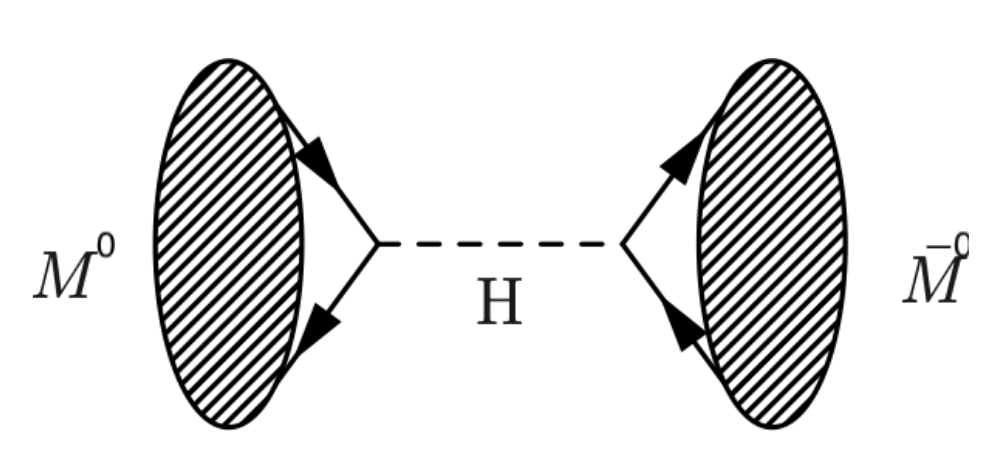
\includegraphics[ width=\textwidth]{placeholder.png}
    \end{minipage}
    \caption{Meson oscillation mediated by a neutral scalar Higgs.}
    \label{fig:3HDM_oscilation_meson}
\end{figure}


While starting at loop-level we have the $\chi_s \gamma$ channel. The quark level transition occurring here is, $b \rightarrow s \gamma$. Without getting in depth at how these processes are calculated, we show the Feynman diagrams where this process happen,

\begin{figure}[H]
%
\begin{minipage}{.5\linewidth}
\centering
            \begin{fmffile}{feyngraph_3HDM_11}
            \begin{fmfgraph*}(100,60)
            \fmfstraight
            \fmfleft{i1,i2}
            \fmfright{o1,h,o2}
            \fmf{fermion}{i1,t1} 
            \fmf{fermion}{t2,i2}
            \fmf{fermion,label=$u_i$}{t3,t2}
            \fmf{fermion,label=$\bar{u}_i$}{t1,t3}
            \fmf{dashes,label=$H^-$}{t1,t2} 
            \fmf{dashes}{t3,h}
            \fmflabel{$\bar{s}$}{i1}
            \fmflabel{$b$}{i2}
            \fmflabel{$\gamma$}{h}
            \end{fmfgraph*}
            \end{fmffile}
\end{minipage}
%
\begin{minipage}{.5\linewidth}
\centering
            \begin{fmffile}{feyngraph_3HDM_12}
            \begin{fmfgraph*}(100,60)
            \fmfstraight
            \fmfleft{i1,i2}
            \fmfright{o1,h,o2}
            \fmf{fermion}{i1,t1} 
            \fmf{fermion}{t2,i2}
            \fmf{fermion,label=$u_i$,tension=1.0}{t1,t2}
            \fmf{dashes,label=$H^+$,tension=1.0}{t1,t3}
            \fmf{dashes,label=$H^-$,tension=1.0}{t2,t3} 
            \fmf{dashes}{t3,h}
            \fmflabel{$\bar{s}$}{i1}
            \fmflabel{$b$}{i2}
            \fmflabel{$\gamma$}{h}
            \end{fmfgraph*}
            \end{fmffile}
\end{minipage}\par\medskip
%
\centering
\begin{minipage}{.5\linewidth}
\centering
            \begin{fmffile}{feyngraph_3HDM_13}
            \begin{fmfgraph*}(100,60)
            \fmfstraight
            \fmfleft{i1,i2}
            \fmfright{o1,h,o2}
            \fmf{fermion}{i1,t1} 
            \fmf{fermion}{t2,i2}
            \fmf{fermion,label=$d_i$}{t3,t2}
            \fmf{fermion,label=$\bar{d}_i$}{t1,t3}
            \fmf{dashes,label=H}{t1,t2} 
            \fmf{dashes}{t3,h}
            \fmflabel{$\bar{s}$}{i1}
            \fmflabel{$b$}{i2}
            \fmflabel{$\gamma$}{h}
            \end{fmfgraph*}
            \end{fmffile}
\end{minipage}\par\medskip
\caption{NP contribution to the transition mediated by a charged or neutral Higgs at loop order as to contribute to $\mathcal{BR} \rightarrow \chi_s \gamma$ trough $b \rightarrow \bar{s} \gamma$ }
\label{fig:3HDMChiSGamma}
\end{figure}

\subsubsection{Review}

As quick general revision of the methodology introduced in the B-L-SM section, recall that any BSM theory must allow for consistency with the SM. 
%
This, especially for multiscalar models, requires checking a large numbers of bounds that are imposed on the complex parameter space. 
% 
Given the large scalar content of the 3HDM, this begins by giving special attention to the possibility of the scalar potential becoming unbounded-from-below.
%
Some necessary conditions are easy to find, looking at Eq. \ref{eq:3HDM_Scalar_Pot}, such as the following couplings being positive so that the potential does not tend towards $-\infty$ when the squared fields become large. 
%
\begin{equation}
\lambda_1 > 0  \quad , \quad \lambda_2 > 0 \quad , \quad \lambda_3 > 0 \quad , 
\end{equation}
%
To further find the proper conditions we must follow a procedure similar to the one used in the 2HDM \cite{Branco_1996}.
%
By taking two doublets pairs at a time $(i, j)$ to infinity but such that ensuring that $\phi_i^\dagger \phi_j = 0$ (which is easily accomplish-able, if for one doublet the upper components are zero and for the other one the lower components vanish) one obtains a positive value of the potential for any value of the fields if,
%
\begin{equation}
\lambda_4 > -2 \sqrt{\lambda_1 \lambda_2} \quad , \quad \lambda_5 > -2 \sqrt{\lambda_1 \lambda_3} \quad , \quad \lambda_6 > -2 \sqrt{\lambda_2 \lambda_3}
\end{equation}
%

We can also adapt the bounded-from-below necessary conditions from ref. \cite{Moretti_2015} (their expressions 21–24), while considering the fact that the potential of that work is different from ours and making the necessary adjustments. 
%
This translates into a generalisation of the above conditions, which become
%
\begin{equation}
\begin{gathered}
\lambda_4 > - 2 \sqrt{\lambda_1 \lambda_2} - \text{min}(0,\lambda_7) \quad , \quad  \lambda_5 > -2 \sqrt{\lambda_1 \lambda_3} - \min(0,\lambda_8 - 2\|\lambda_{10}\|)  \\
\lambda_6 > - 2 \sqrt{\lambda_2 \lambda_3} - \min(0,\lambda_9) \quad . 
\end{gathered} 
\end{equation}
%
These conditions eliminate a great deal of parameter space, and though they are not sufficient ones, they should cover most of the parameter space leading to an unbounded-from-below potential.

Other bounds like the upper perturbatively bound, ensuring all scalar couplings $\lambda_{1,10}$ are maintained bellow $4\pi$.

As for constraining the unitarity, we again leave the calculation of the scattering amplitudes of scalar-scalar elastic interactions to SPheno. 
%
In multiple Higgs models this is done by the diagonalization of the S-matrix (S for scattering), comprised of all these amplitudes.
%
Once diagonalized, it can be checked for unitarity, and ensure that at high energies we respect the optical theorem {\color{red} do I need a citation or explain? is this too much?}. 

This could be done manually by following a process like seen in Ref\,\cite{Moretti_2015}, however it is far more convenient to leave this job for SPheno. 

Finally, a standard constraint on multiscalar models is to verify their compliance with electroweak precision bounds or STU bounds, see Ref\,\cite{Peskin1992} { \color{red} which chapter?}. 
% 
Models with N Higgs doublets automatically satisfy $\rho = 1$ at tree-level, meaning bounds on the oblique parameter S will be easily satisfied. These parameters are also calculated by SPheno. 

%However we now have the additional constraint coming from our flavour analysis trough the discussed QFV observables. 
%

\subsection{Discussion of results}

The main objective of our work was to design a tool with whom we can probe large and complicated parameter spaces of BSM models as discussed previously. 
%
A more advanced version of the previously implemented process was implemented in this 3HDM model.
%
With it we tried to scam over all relevant free parameter space and would like to present the results of said scan in this chapter. 
%
%The central discussion of the scanning apparatus will focus on the new flavour constrictions and the inversion process.  
%
With it we find the parameter space that not only respects all scalar and EW analysis as implemented on the B-L-SM model, but also keeps all examined QFV observables within the 2 $\sigma$ deviation limit and ensures the proper invesion process. 
% we can take from a random 3HDM scan with flavour as a chief constricting factor. All flavour observables were kept within the 2 $\sigma$ limit.

We already touched on how Higgs physics can be detected on large collider experiments and how flavour can also limit our searches as strong interactions of quarks trough the exotic Higgs could lead to excess quark violation. % forget the additional EW precision observables that also play a key role in excluding large parts of the available paramater space. 
%
The process we undertook here was exactly the same as we performed on the B-L-SM discussed in section \ref{sec:later}. 

We can see the S, T and U variables for our parameter space in the following Figs, 
%
\begin{figure}[H]
	\centering
	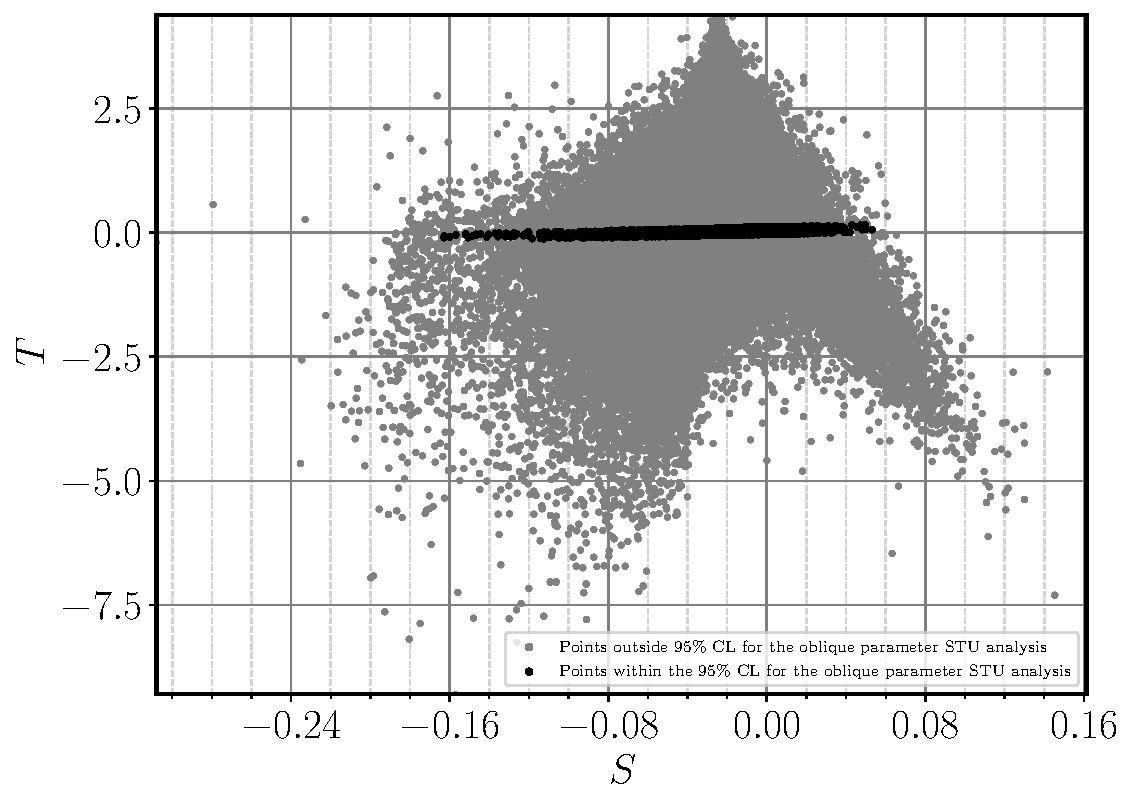
\includegraphics[width=.49\textwidth]{Images/3HDM/EW/EW_S_T_black.pdf}	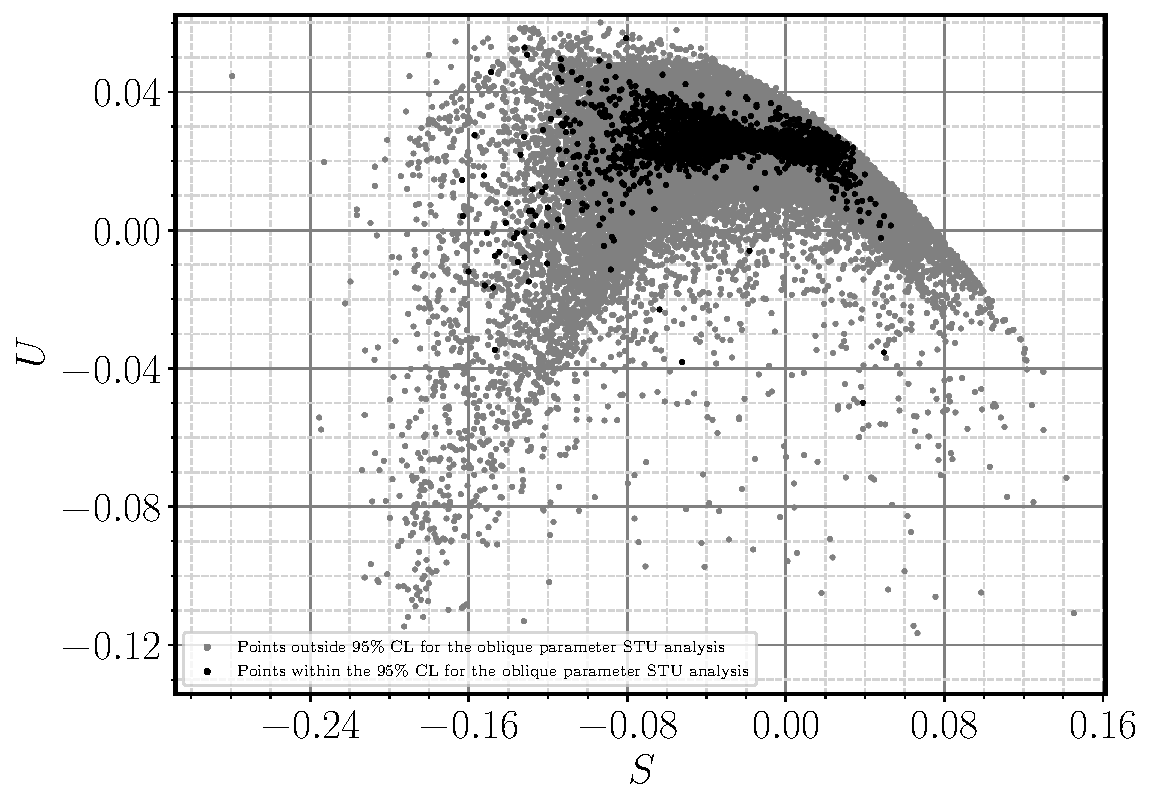
\includegraphics[width=.49\textwidth]{Images/3HDM/EW/EW_S_U_black.pdf}
	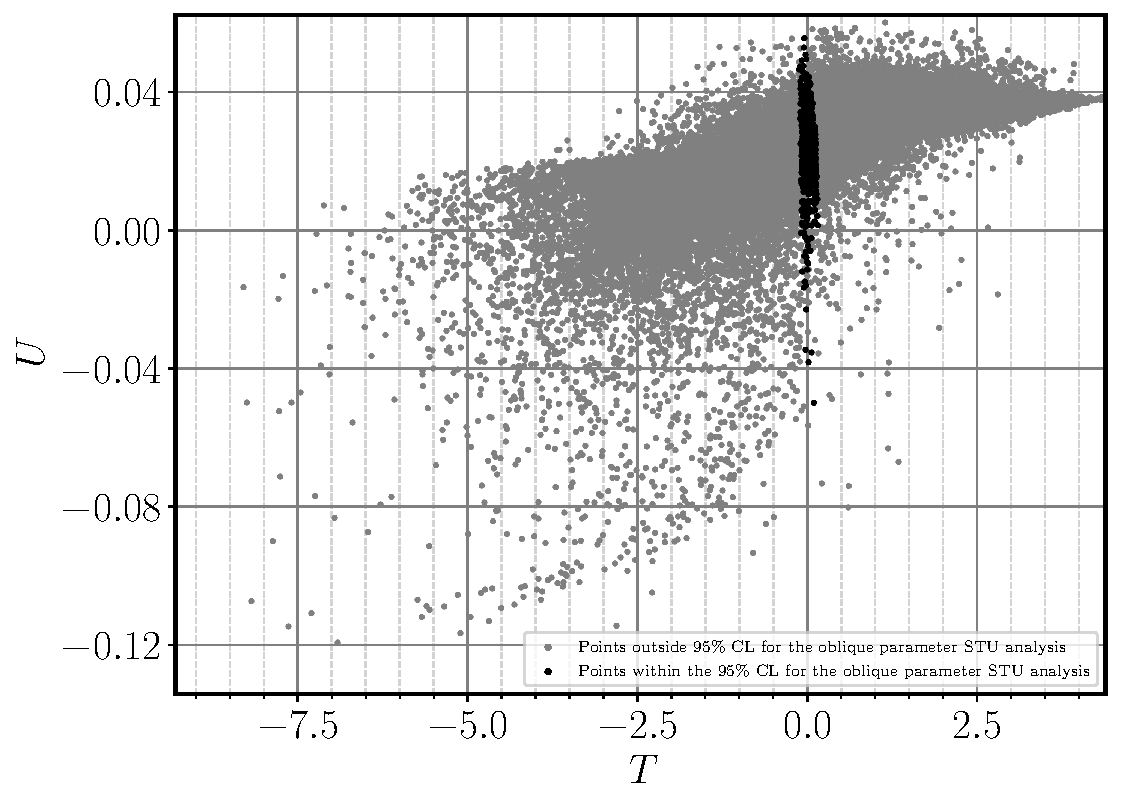
\includegraphics[width=.49\textwidth]{Images/3HDM/EW/EW_T_U_black.pdf}
	\caption{}
	\label{Fig:3HDM_STU}
\end{figure}	
%
We can clearly see that NP can have a very strong effect on some of these observables, most notably in the deviation in the T variable.
%
Note that this variation makes the elipsoid seen previously look like a narrow region. 
%
As in the B-L-SM the values for $(\Delta S , \Delta T , \Delta U )$ are taken from  Ref\,\cite{Baak_2012}.

% Meantion :  In order to test the obliqueparameters, we implement results for the SM fit from the Gfitter collaboration [45].   %  M. Baak, M. Goebel, J. Haller, A. Hoecker, D. Ludwig, K. Moenig et al.,UpdatedStatus of the Global Electroweak Fit and Constraints on New Physics,Eur. Phys. J.C72(2012) 2003 [1107.0975] 

The STU results discussed we can continue our work by showing the available corresponding physical parameter space. 
%
Recall that our inversion process logarithmic scanned over the 16 real parameters in this space, the scalar masses, soft breaking terms and all mixing angles.  
%
For brevity we will present our results only in order to the scalar masses,
%We can begin by observing the available scalar space. 
%
%Let us describe regions for masses and VEVs that are allowed by Higgs data constraints and EW precision tests. 
%
It is important to mention that the labeling of the scalars is arbitrary, we just ensure that the scalars are labeled in growing mass order e.g. $m_{H^\pm_2} > m_{H^\pm_1}$. 
%
This change does not have any real physical significance but it leaves our graphs with a linear cut where $m_i = m_j$. 
%
One important characteristic of our results worth discussing is the presence of relatively light  scalars.
%
\begin{figure}[H]
	\centering
	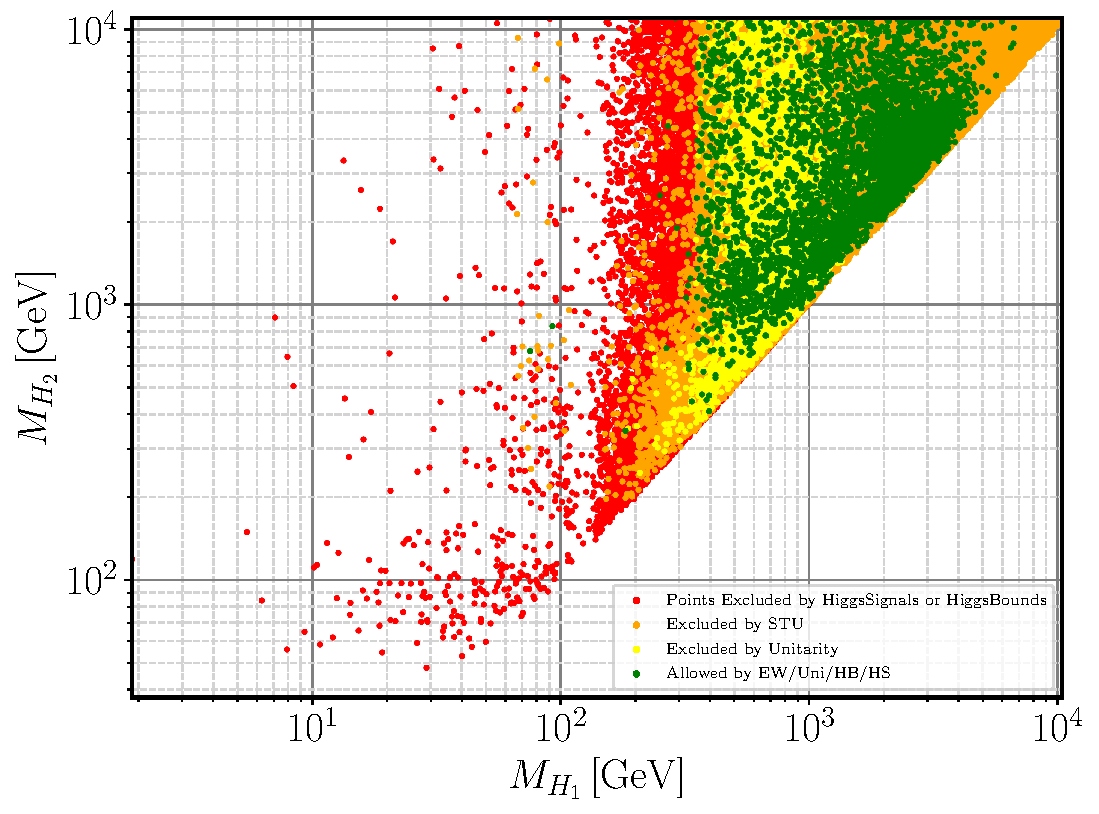
\includegraphics[width=.49\textwidth]{/3HDM/H1_H2.pdf}
	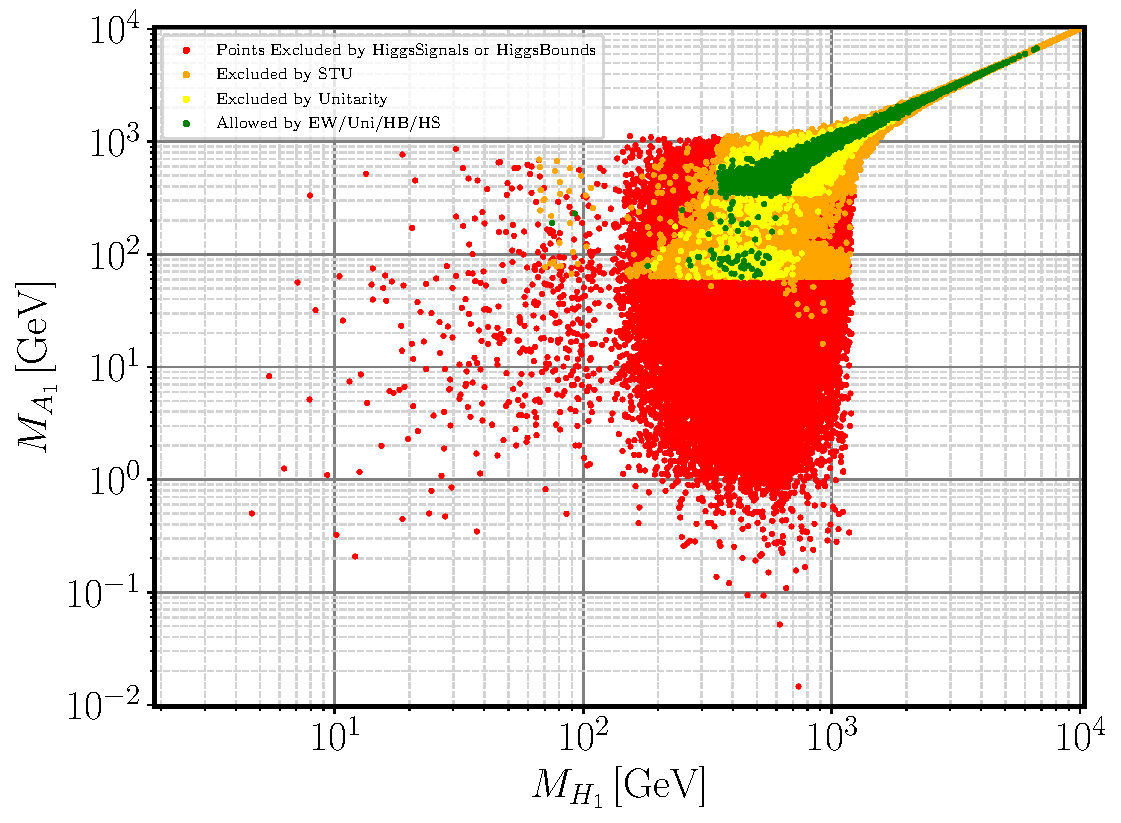
\includegraphics[width=.49\textwidth]{/3HDM/H1_A1.pdf}
	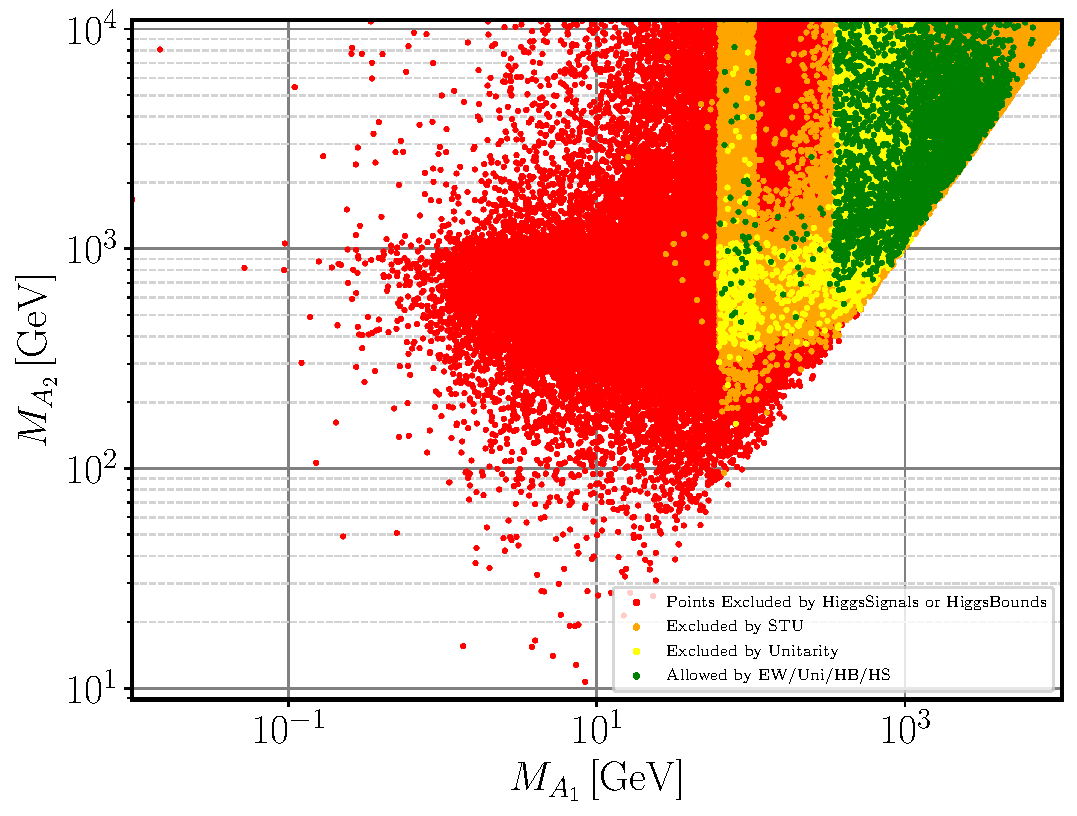
\includegraphics[width=.49\textwidth]{/3HDM/A1_A2.pdf}
	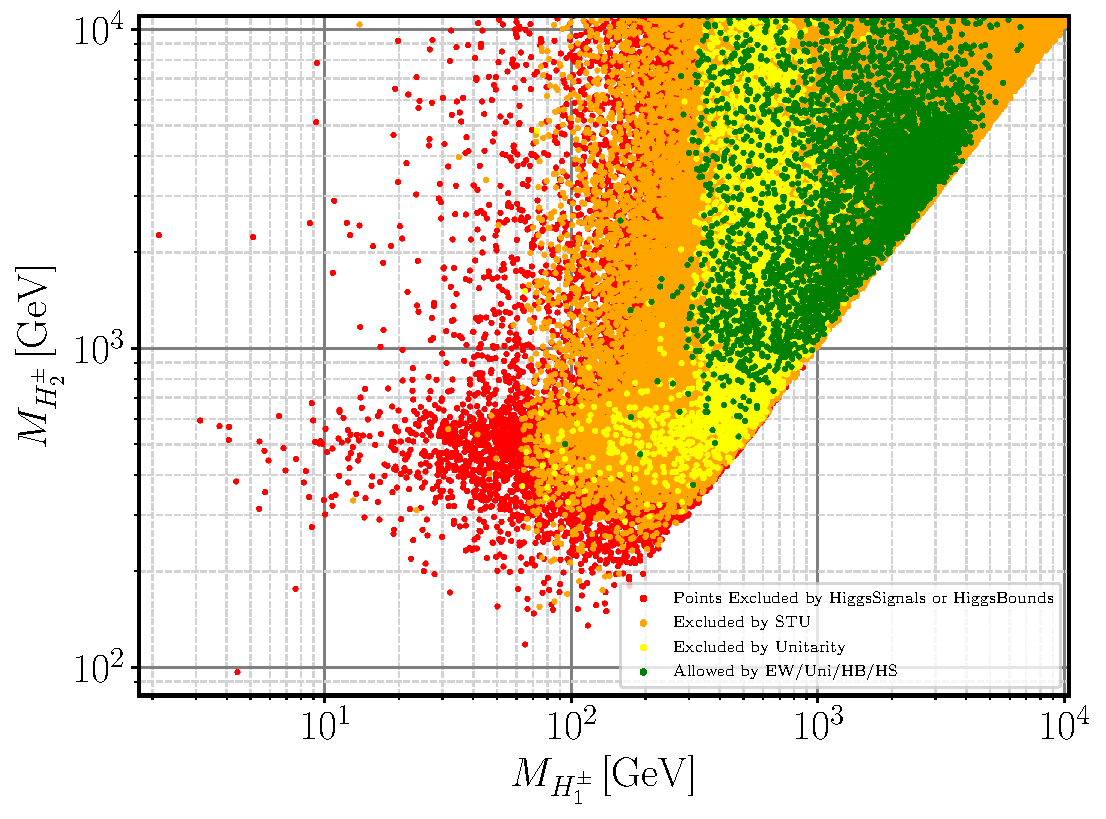
\includegraphics[width=.49\textwidth]{/3HDM/Hc1_Hc2.pdf}
	\caption{Scatter plots of parameter space allowed under several cuts imposed on the BGL-like 3HDM. On the upper right side we have the plot showing the masses of the two heavier CP-even scalars $H_2$ and $H_1$ while in the right we show the relation between the lightest (non SM Higgs) of the CP-even and pseudoscalar particles. As for the bottom plots see the remaining CP-odd scalars and how they are excluded under several cuts. Right we have the pseudoscalar masses $A_1$ and $A_2$ while in the left side we have the CP- odd charged Higgs states $H_1^\pm$ and $H_2^\pm$.	Red points failed HS and HB tests; yellow points violate unitarity constraints; orange points only fail electroweak precision constraints, and green ones satisfy all restrictions.}
	\label{fig:H1_A1_Plots}
\end{figure}	

One important characteristic of our results worth discussing is the presence of relatively light  scalars. 
%
And we can see that there is clearly defined zones where HiggsBounds and HiggsSignals allow scalars to exist. 
%
Next there is a zone within where STU limits are fulfilled at 95 \% C.L. and within that zone we see that only a small region respects unitarity constraints. 
%
We can then argue that our model predicts the existence of masses around (300's GeVs check in detail later) which are in harmony with the SM i.e. are so far compatible with observations. 


{ \color{red} why do pseudo scalar masses tend to funnel? } 

Note that, by requiring that we have a SM-like Higgs boson, naturally imposes conditions upon the couplings of the heavier (or lighter) CP-even scalar states to the Gauge bosons, and seeing that the harshest condition on most scalar sectors is the di-Z production we then have that due to the alignment limit imposed the majority of the scalar sector is allowed. 

We can also see that unless the signal coming from the pseudoscalar masses is masked by the Higgs SM signal or the pseudoscalar is heavy (in the TeV region) that it poses a harsh cut on the parameter space.

 { \color{red} Why then are the pseudoscalars so constricted. }   

\subsubsection{Flavour Cuts }

% Having shown that there are no instances of heavy fine tuning in our model. 

Before showing what combined regions we observe stemming from the cuts discussed above when combined with QFV observables, it might be a worth while endevour to see what type of regions we can see with only QFV observables. 
%
First we show what the fractions of QFV observables show,    

\begin{figure}[H]
	\centering
	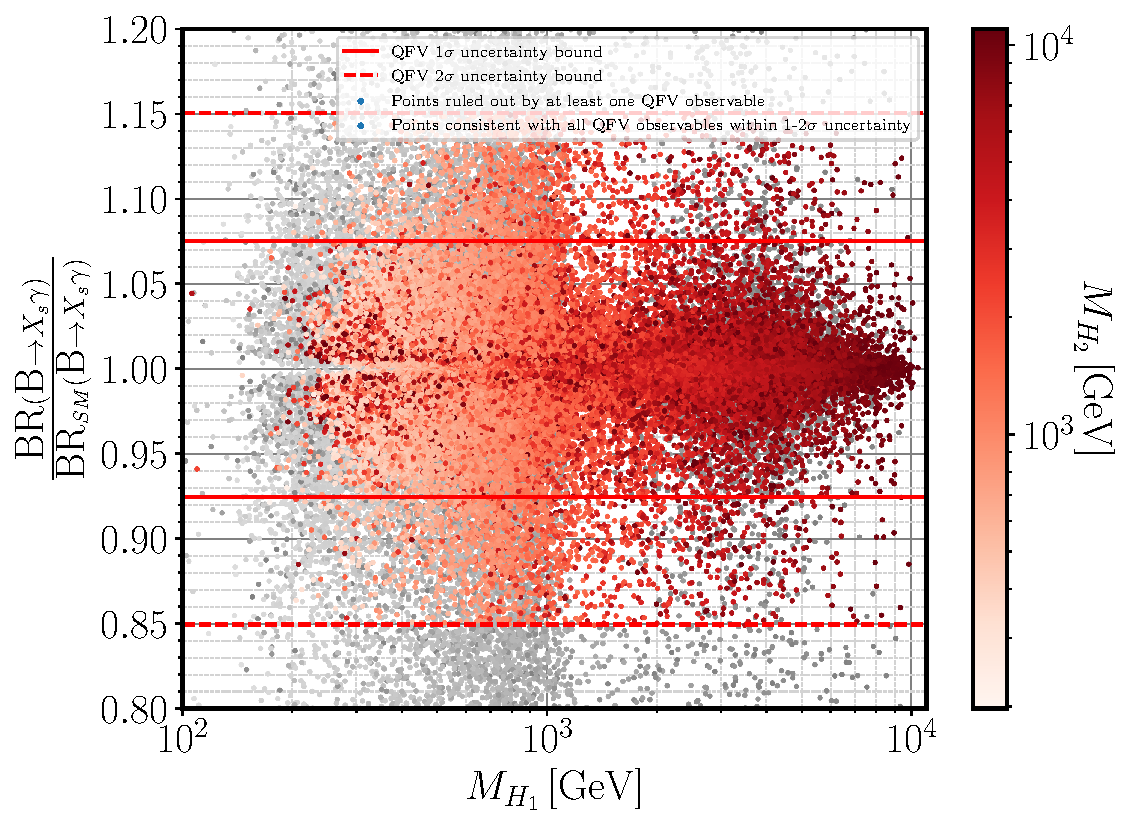
\includegraphics[width=.49\textwidth]{Images/3HDM/Reds/Xsgamma_H1_H2.pdf}
	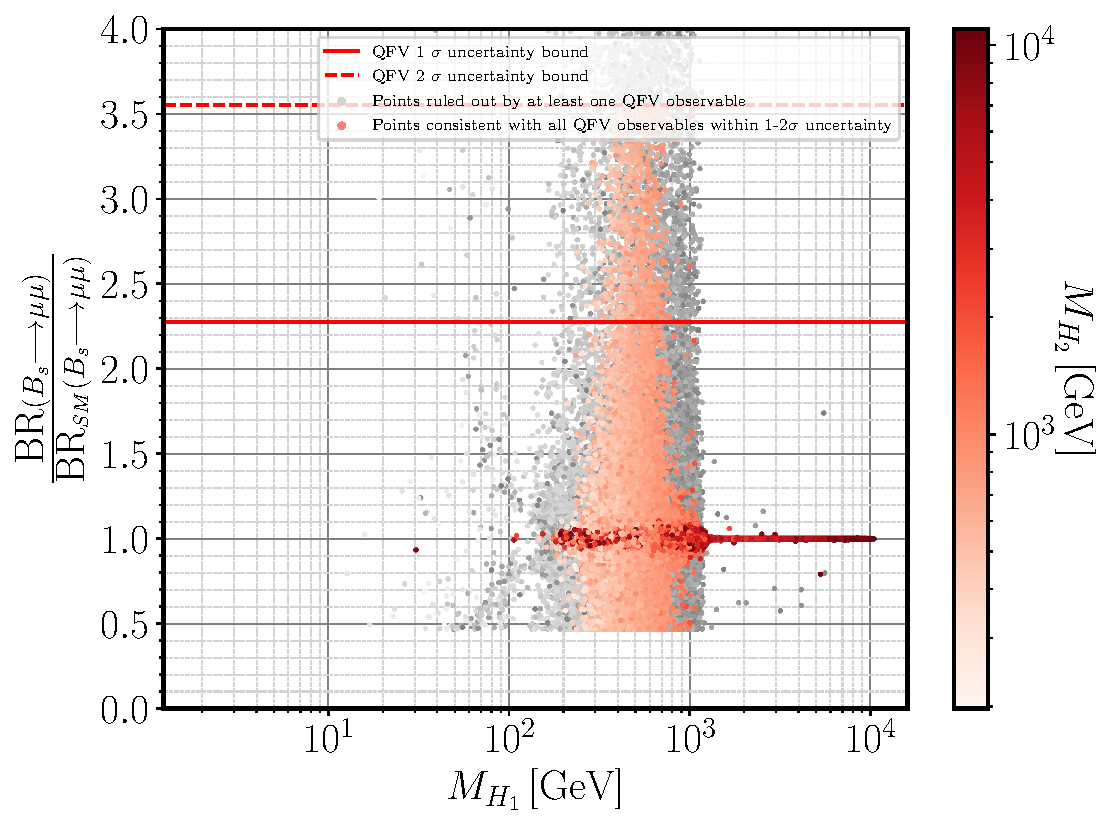
\includegraphics[width=.49\textwidth]{Images/3HDM/Reds/Bsmumu_H1_H2.pdf}
	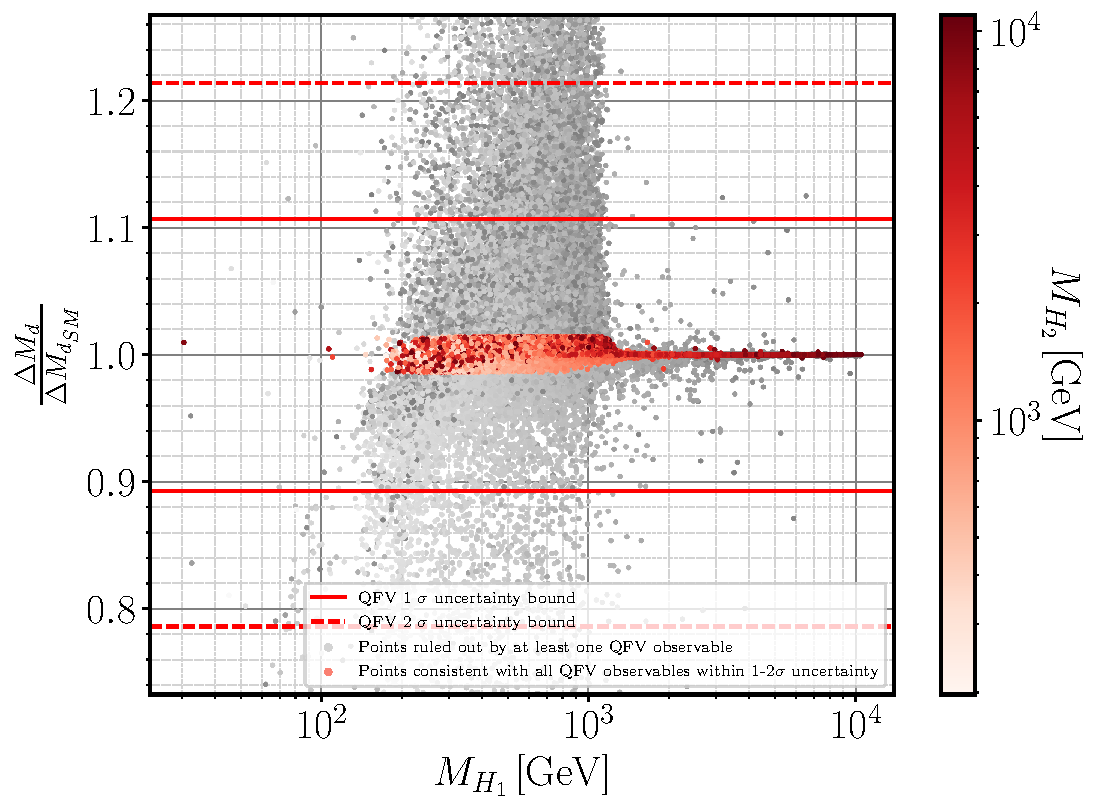
\includegraphics[width=.49\textwidth]{Images/3HDM/Reds/DeltaMd_H1_H2.pdf}
    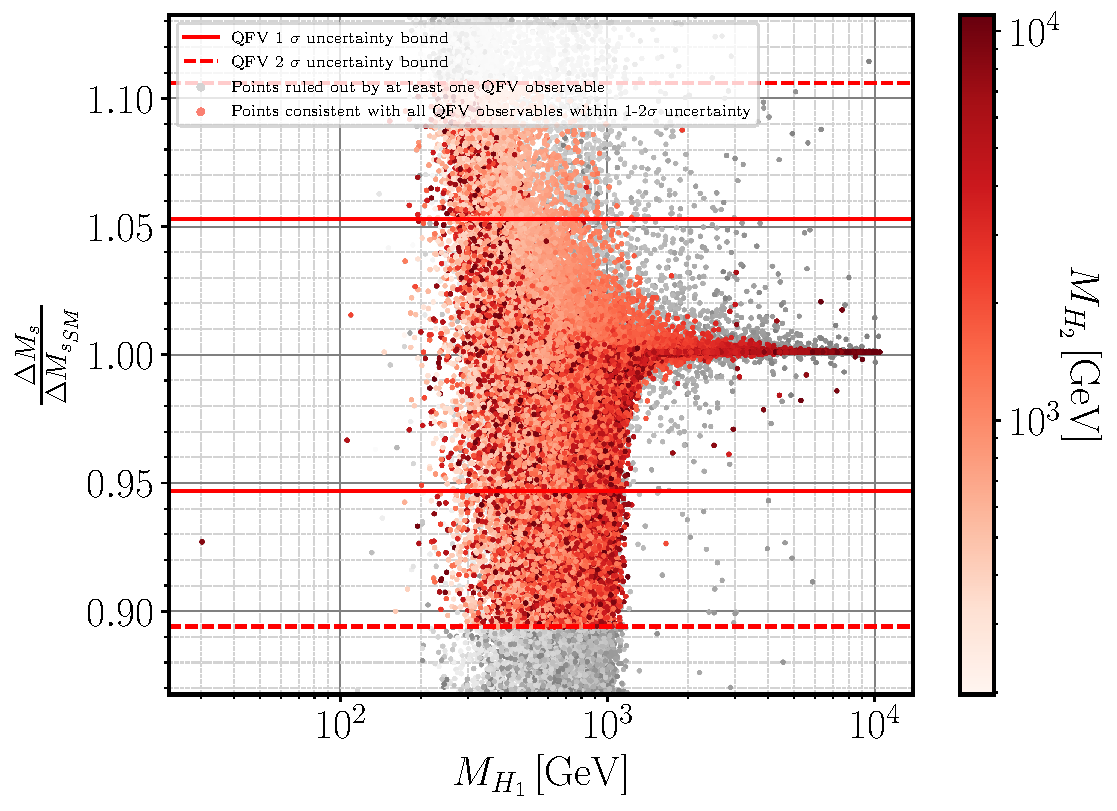
\includegraphics[width=.49\textwidth]{Images/3HDM/Reds/DeltaMs_H1_H2.pdf}
    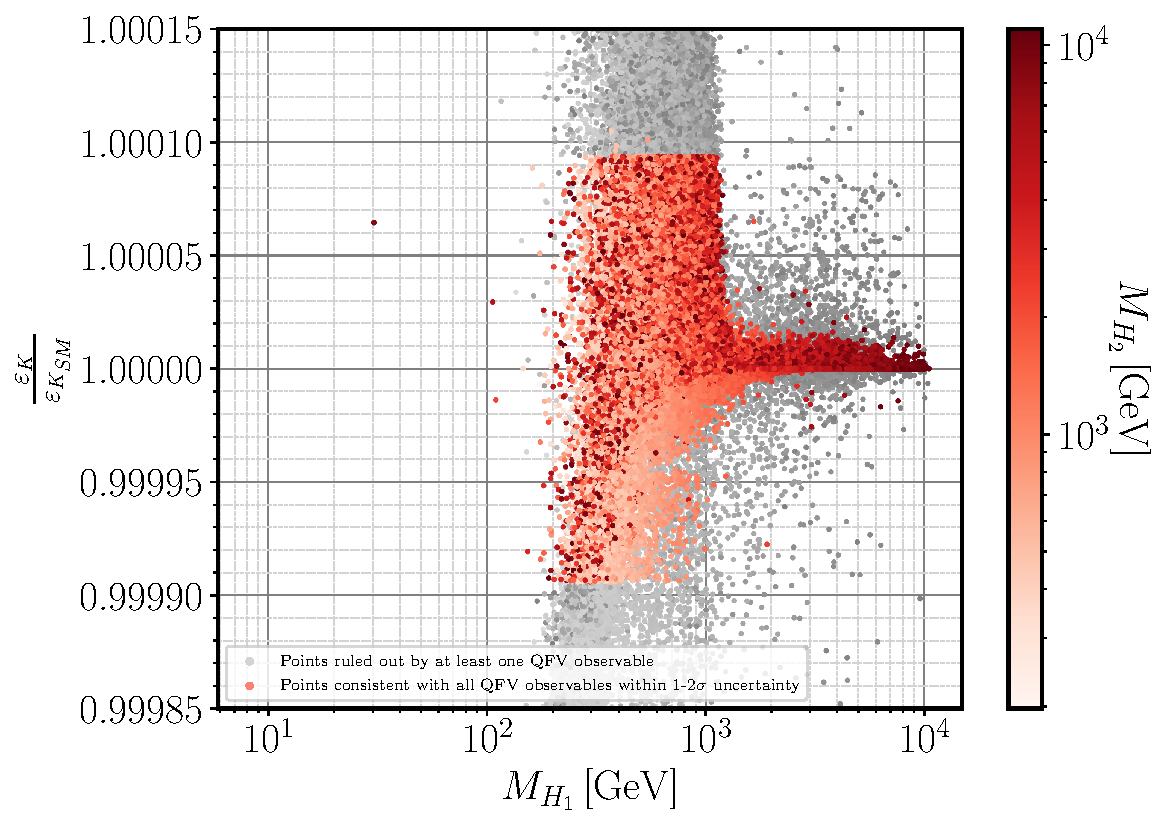
\includegraphics[width=.49\textwidth]{Images/3HDM/Reds/Eps_K_H1_H2_Centered.pdf}
	\caption{ Scatter plot of the estimated QFV observables normalized to the SM values. The grey points in all plots represent a point that would be outside the 2 $\sigma$ bound for one of the observables while in a red color scale we see the second CP-even neutral scalar mass for the remaining points.  }
	\label{fig:3HDM_Flavour}
\end{figure}	

\begin{table}[H]
\centering
\begin{tabular}{lcccccc}
                           & $\frac{\textrm{BR} ( \textrm{B} \rightarrow X_s \gamma)}{\textrm{BR}_{SM} ( \textrm{B} \rightarrow X_s \gamma )}$ 
                           &  $\frac{ \textrm{BR} (B_s  \longrightarrow  \mu  \mu )}{\textrm{BR}_{SM}(B_s  \longrightarrow  \mu  \mu ) }$  
                           & $\frac{\Delta M_d}{\Delta M_{d_{SM}} }$ 
                           & $\frac{\Delta M_s}{\Delta M_{s_{SM}} }$
                           & $\frac{\varepsilon_K}{\varepsilon_{K_{SM}}}$ \\
$1 \sigma$ upper QFV bound &  1.08    &  2.27   &  1.10     &  1.05     &    1.13    \\
$1 \sigma$ lower QFV bound &  0.91    &  0.00   &  0.91     &  0.95     &    0.87    \\
$2 \sigma$ upper QFV bound &  1.15    &  3.55   &  1.21     &  1.10     &    1.27    \\
$2 \sigma$ lower QFV bound &  0.85    &  0.00   &  0.79     &  0.90     &    0.72           
\end{tabular}
\end{table}

Note the available zone for $\varepsilon_K/\varepsilon_{K_{SM}}$ and some other decays seems quite small, this is due to ${\textrm{BR} ( \textrm{B} \rightarrow X_s \gamma)}/{\textrm{BR}_{SM} ( \textrm{B} \rightarrow X_s \gamma )}$ and ${\Delta M_s}/{\Delta M_{s_{SM}} }$ being very thightly constraint and the most sensitive in our model.

When combined with the EW and scalar analysis these exclusions wield, 

\begin{figure}[H]
	\centering
	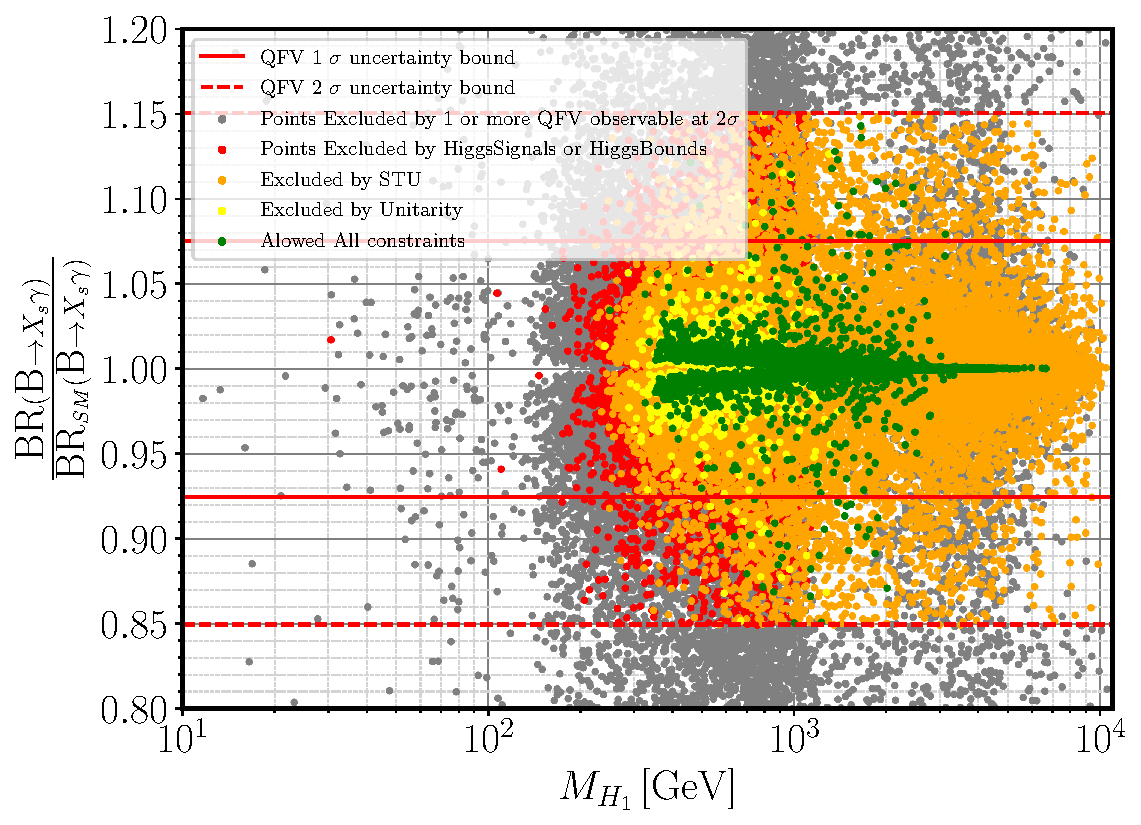
\includegraphics[width=.49\textwidth]{Images/3HDM/PT_Folder/XsGamma_H1.pdf}
	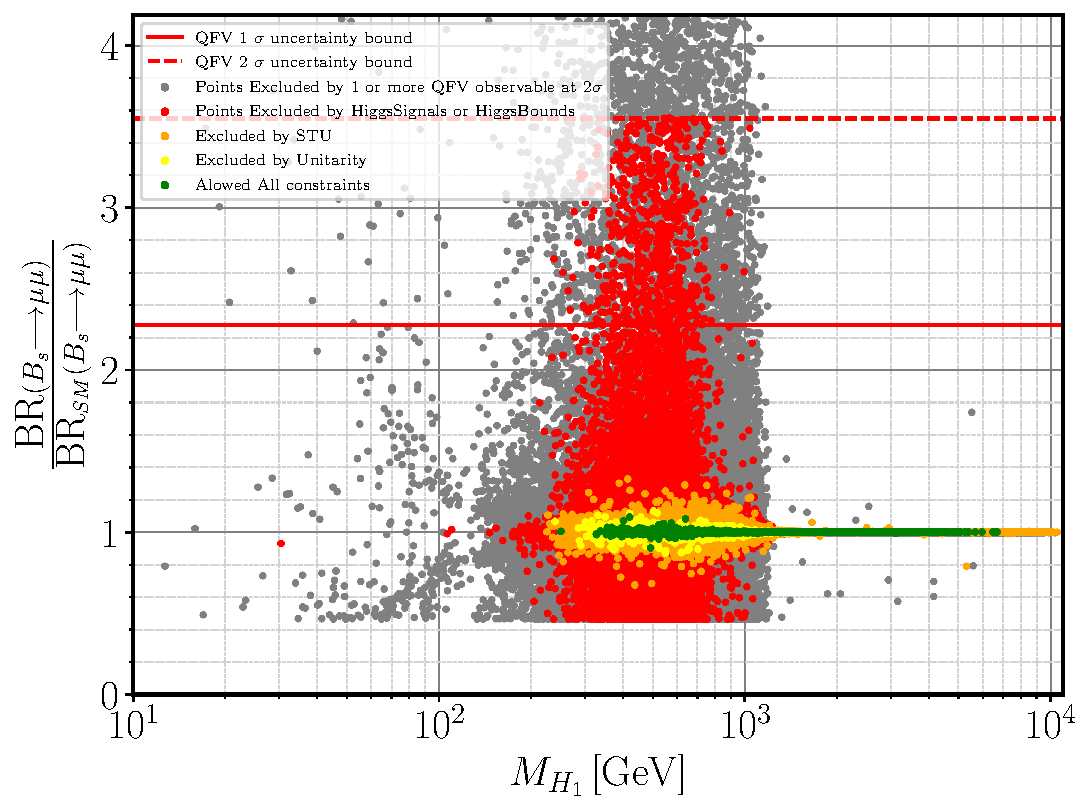
\includegraphics[width=.49\textwidth]{Images/3HDM/PT_Folder/Bsmumu_H1.pdf}	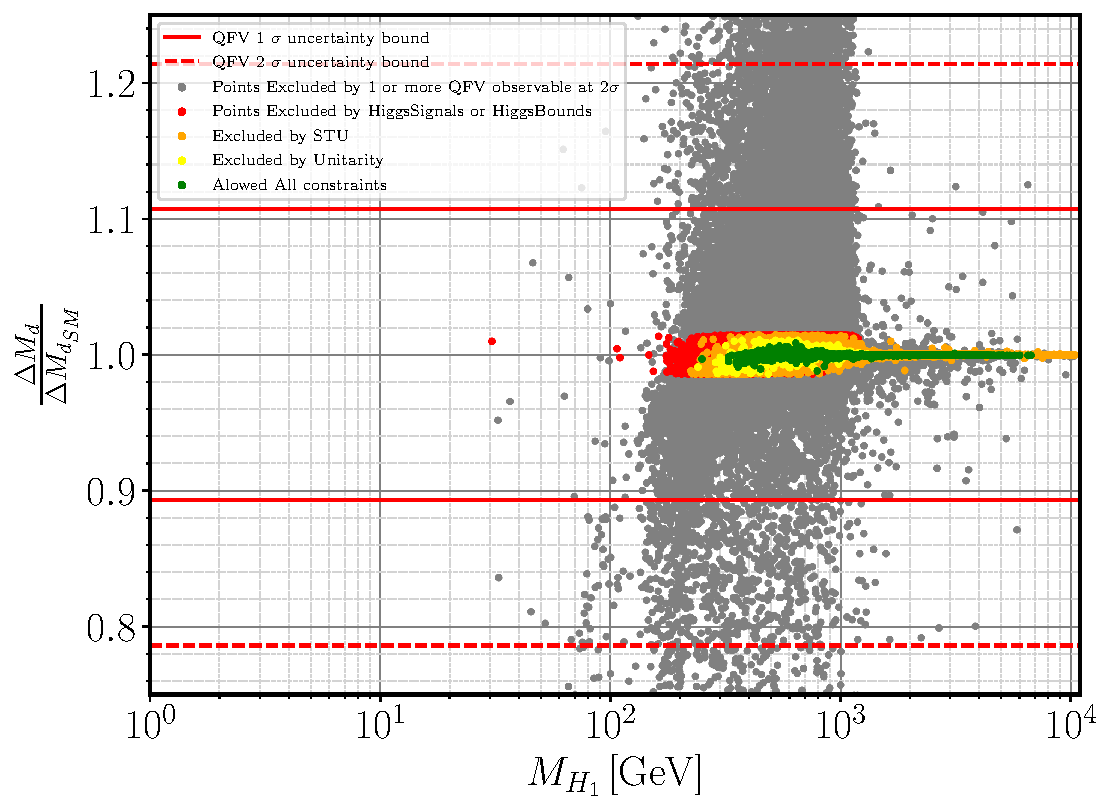
\includegraphics[width=.49\textwidth]{Images/3HDM/PT_Folder/Delta_Md_H1.pdf}
    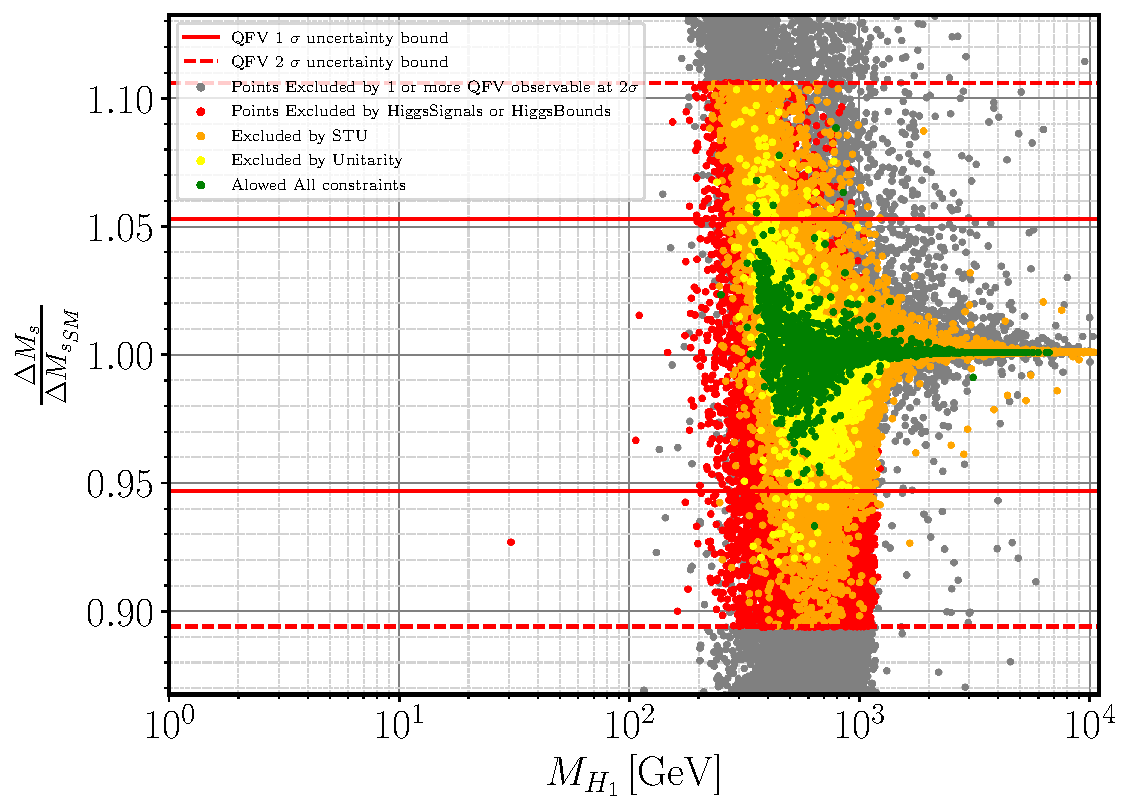
\includegraphics[width=.49\textwidth]{Images/3HDM/PT_Folder/Delta_Ms_H1.pdf}
    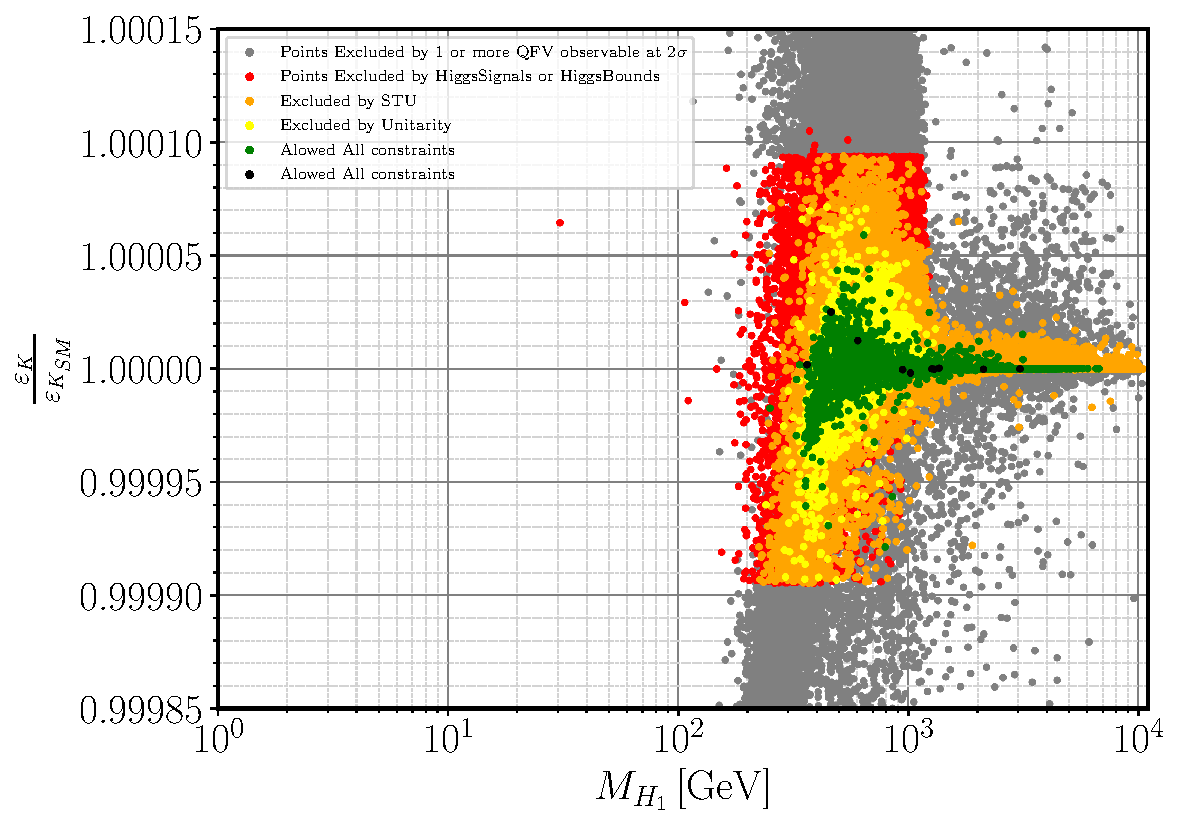
\includegraphics[width=.49\textwidth]{Images/3HDM/PT_Folder/Eps_K_H1_Thighter_Centered.pdf}
    \caption{ Scatter plot of the estimated QFV observables normalized to SM values overlaped with EW and Higgs sector just as in previous figures. } 
	\label{fig:3HDM_Flavour_PT}
\end{figure}	

Here you can clearly see that there is a central region where the points that verify all EW and scalar constraints are almost all also consistent with QFV observables. 

From here we can extract the minimum and maximum measured masses found in our study seen in Tab.\,\ref{Tab:BadTable}.

\begin{table}[H]
\centering
\begin{tabular}{ccccccc}
                            & $H_1$ & $H_2$ & $A_1$ & $A_2$ & $H_1^\pm$ & $H_2^\pm$ \\
$\text{Max}_M (\text{GeV})$ & 6664  & 10979 & 6683  & 10995 & 6623      & 10989     \\
$\text{Min}_M$              & 251   & 412   & 87    & 395   & 157       & 374      
\label{Tab:BadTable}
\end{tabular}
\end{table}

As we meantioned in our opening sections, sometimes in this model it is required some degree of fine tunning as to allow for tree-level QFV not to be detected. 
%
Such a routine was not implemented in our analsysis, howeever our scans randomness could have found a syncronicity where flavour observables are fine-tunned by accident. 
%
%It was important to verify fine-tunning as our scans randomness could have found a syncronicity where flavour observables are fine-tunned by accident. 
%
To check this we rechecked all points with slight a variation of masses trough the a 1\% variation of soft breaking terms. 
%
Such a mass variation is expected to lead to variation of the flavour channel decay amplitude. 
%
Trough this exercise we expect to show that a there is no abruptly high variation of masses or QFV observables.
% 
The results can be seen in, 

\begin{figure}[H]
	\centering
	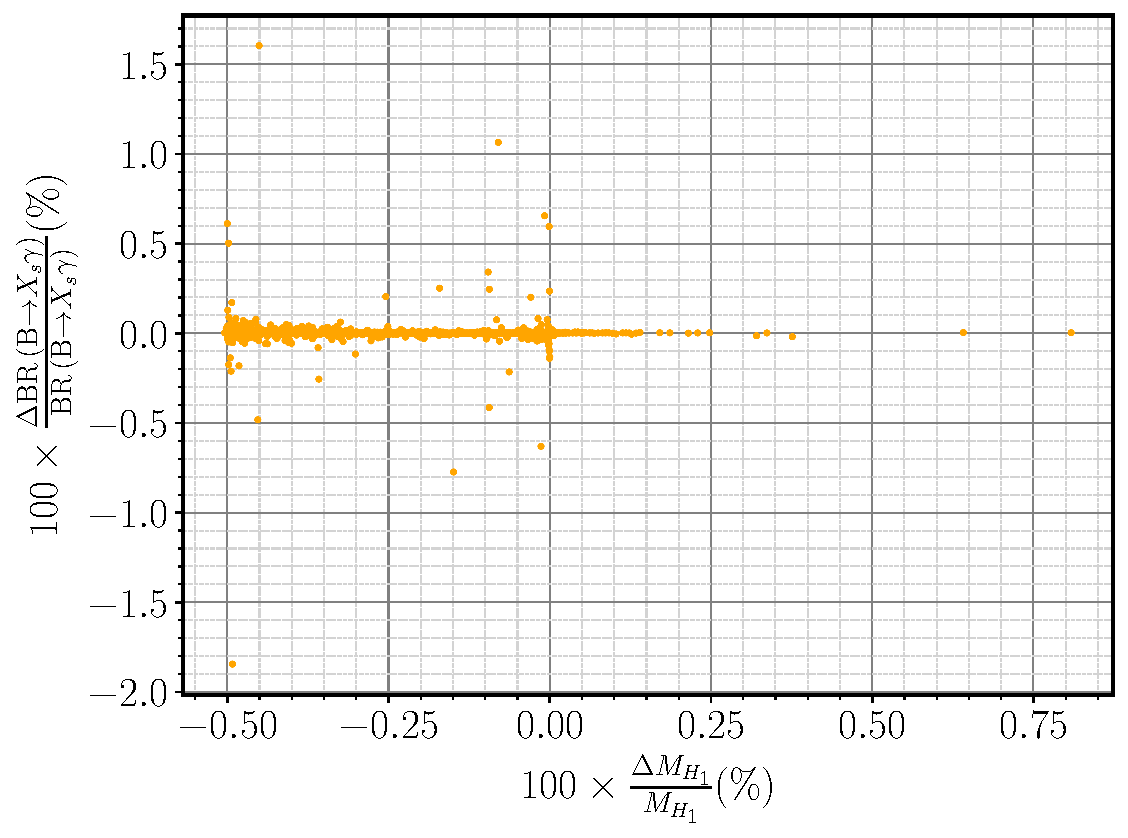
\includegraphics[width=.49\textwidth]{Images/3HDM/Fine_Tuning/Xsgamma_H1.pdf}
	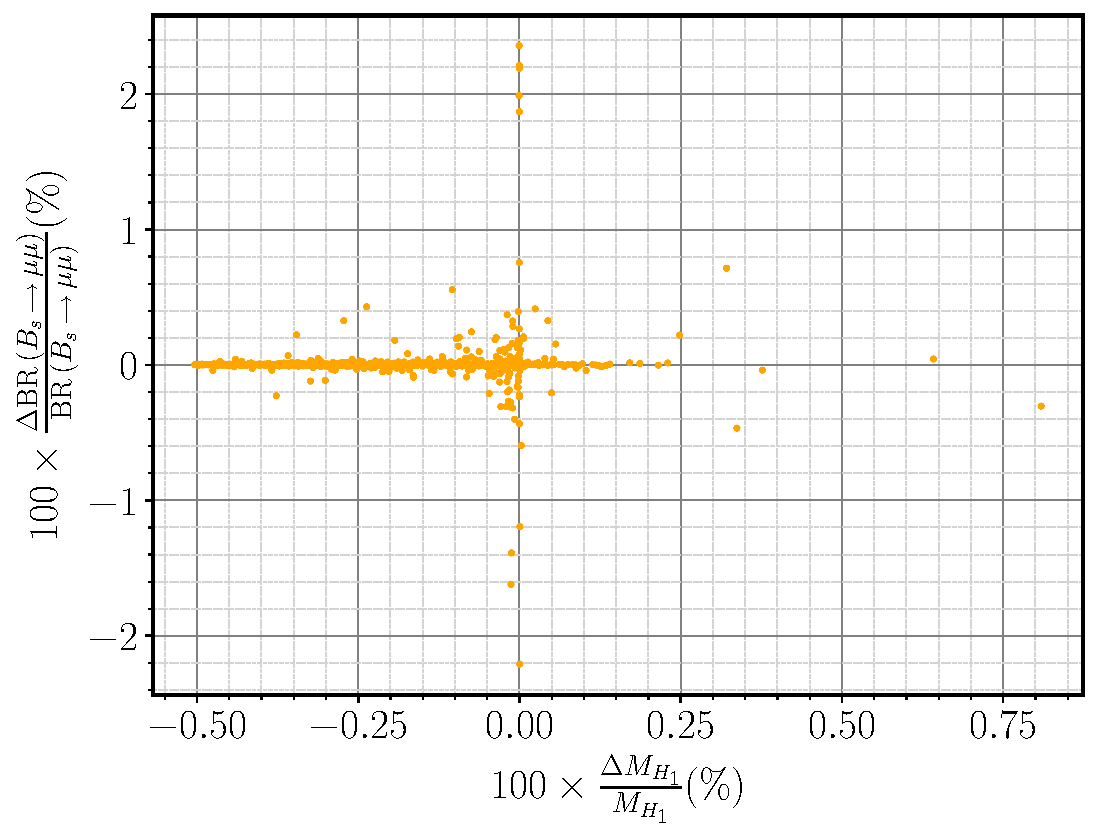
\includegraphics[width=.49\textwidth]{Images/3HDM/Fine_Tuning/Bsmumu_H1.pdf}
	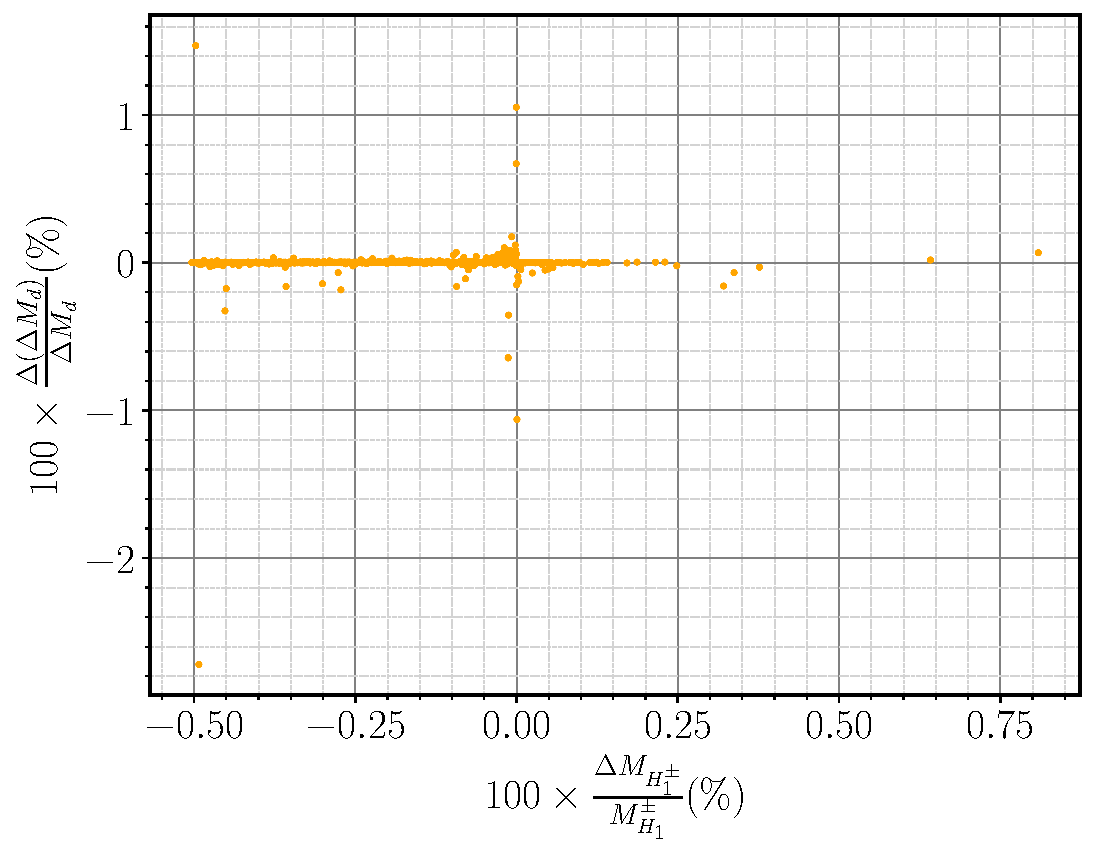
\includegraphics[width=.49\textwidth]{Images/3HDM/Fine_Tuning/DeltaMd_H1.pdf}
    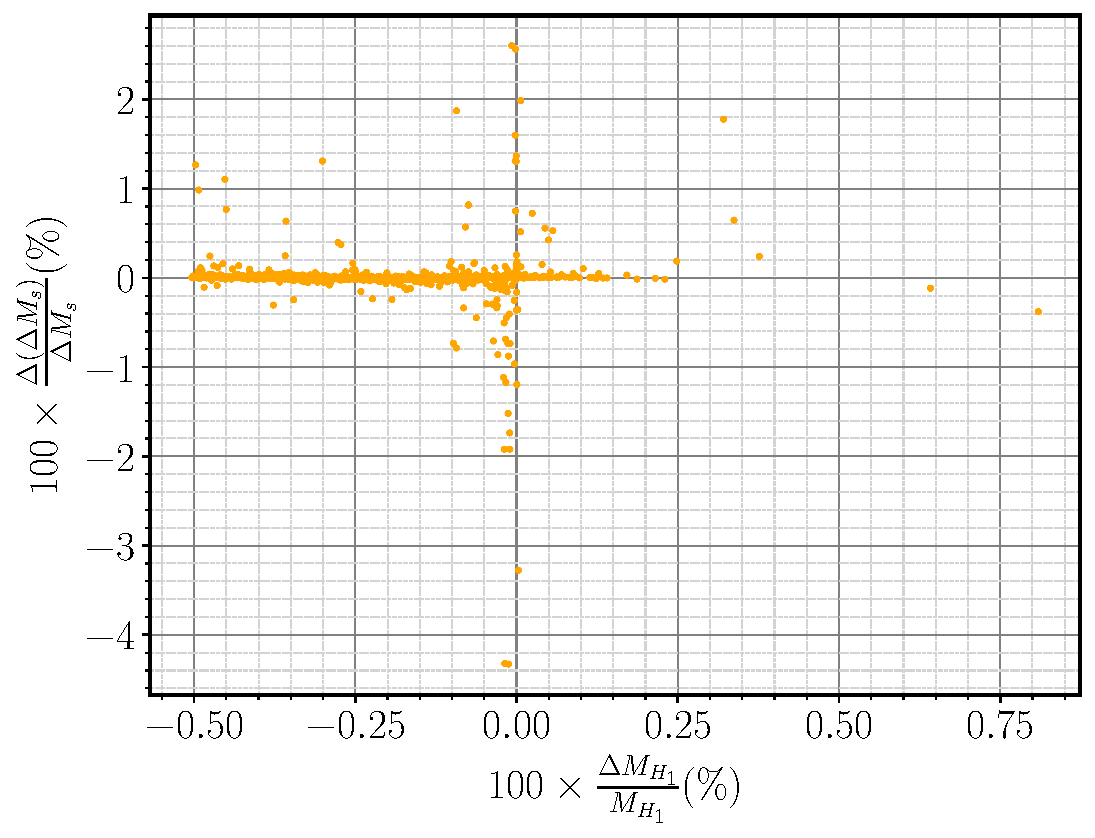
\includegraphics[width=.49\textwidth]{Images/3HDM/Fine_Tuning/DeltaMs_H1.pdf}
    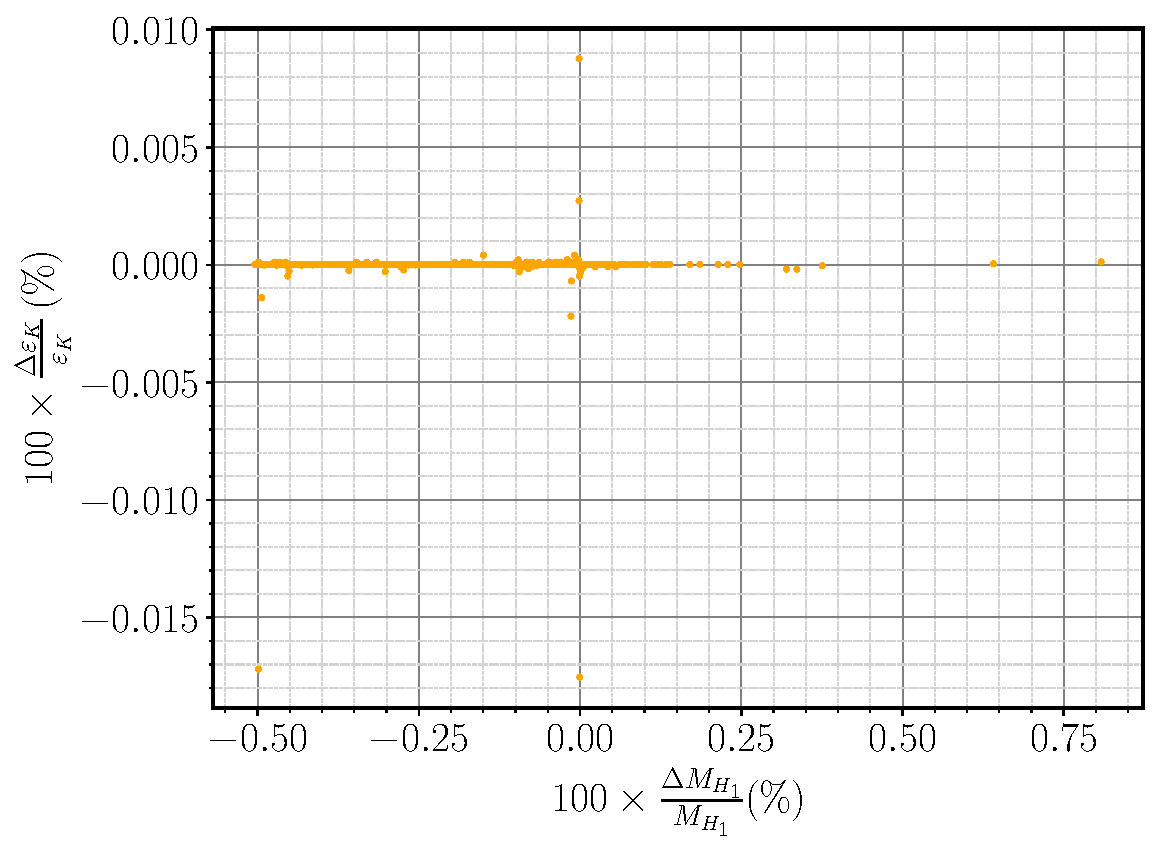
\includegraphics[width=.49\textwidth]{Images/3HDM/Fine_Tuning/eps_K_H1.pdf}
	\caption{Relative mass and QFV observable changes with the increase of 1\% in all softbreaking terms}
	\label{fig:3HDM_Fine_Tunning}
\end{figure}	

Finally a complementary study was also implemented trough Madgraph in this model. 
%
This check was initial performed as to verify if HiggsBounds and HiggsSignals were properly checking gluon fusion channels. 
%
\begin{figure}[H]
	\centering
	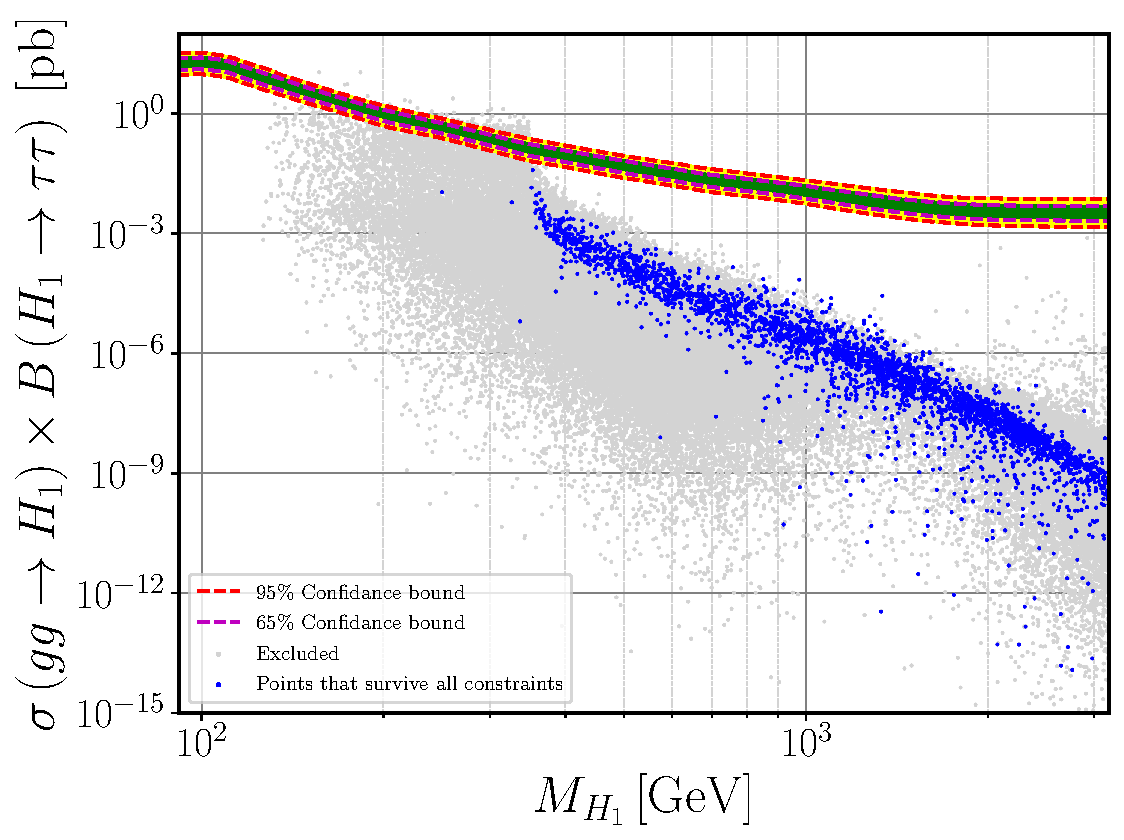
\includegraphics[width=.49\textwidth]{Images/3HDM/Xsec/Xsec_1_Grey_tight.pdf}	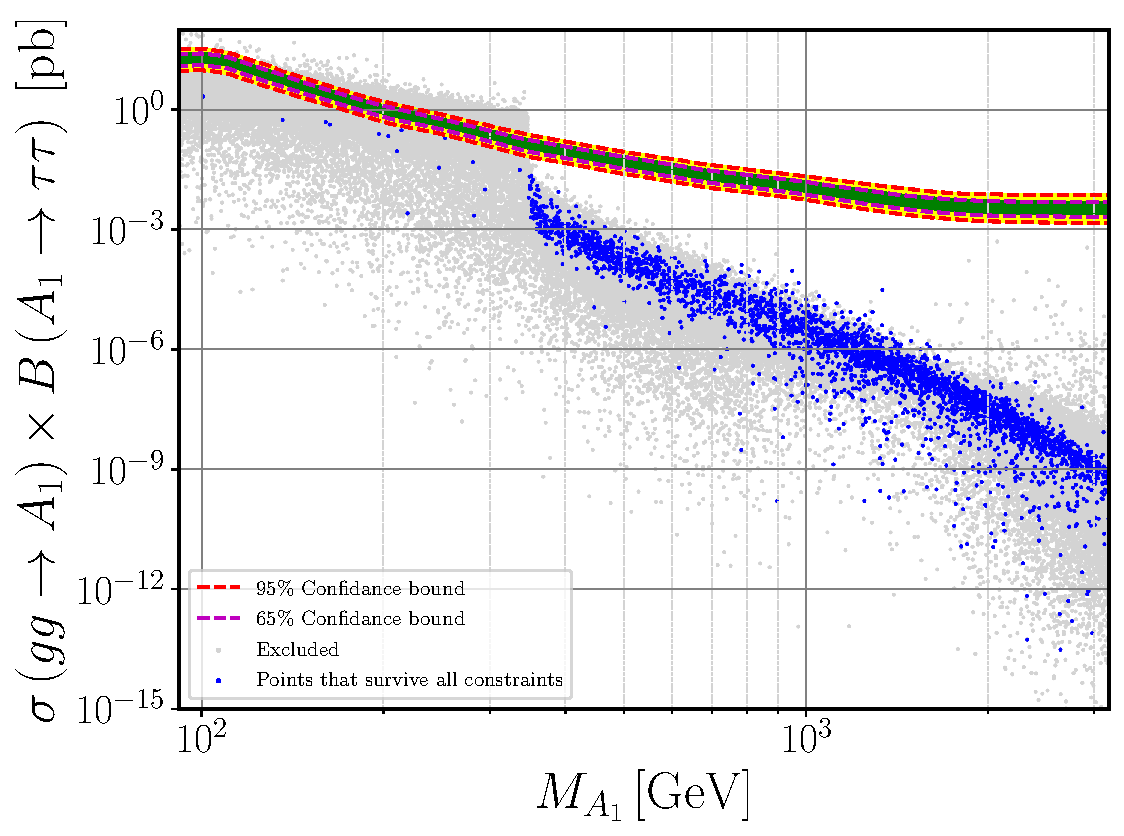
\includegraphics[width=.49\textwidth]{Images/3HDM/Xsec/Xsec_2_Colourful_tight.pdf}
	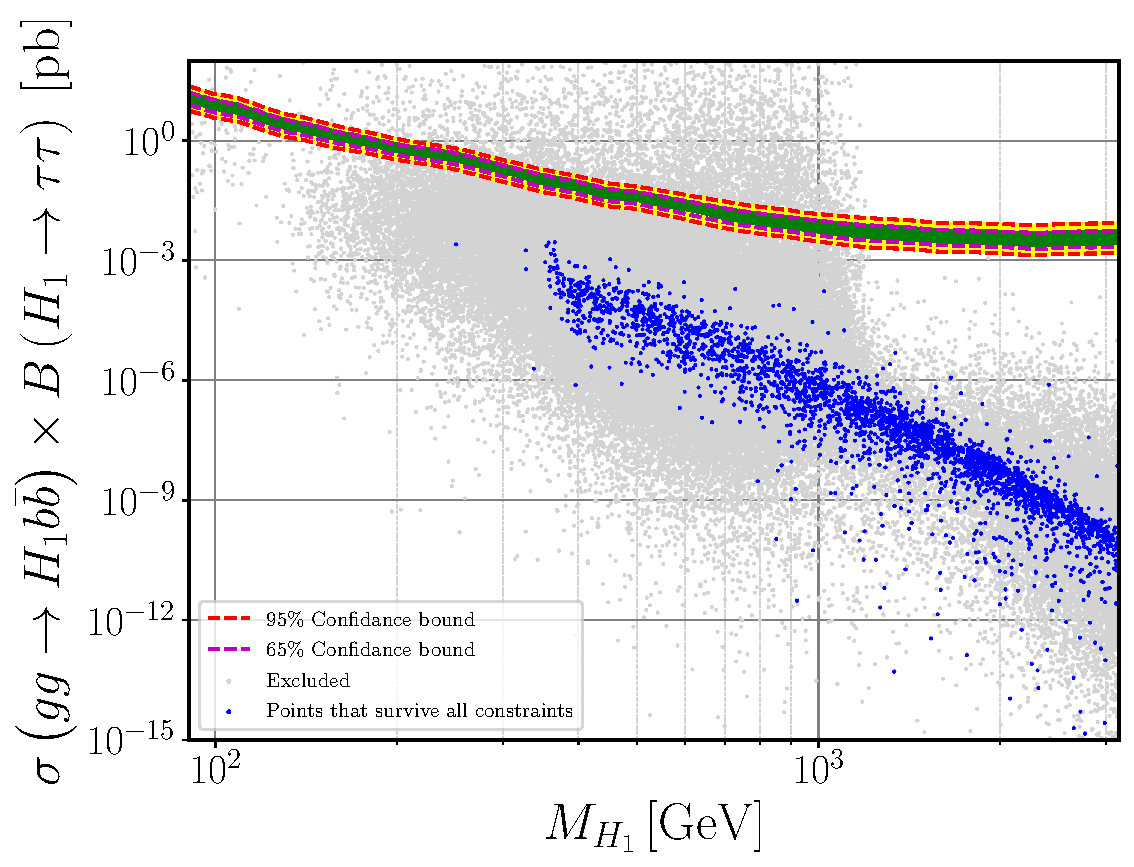
\includegraphics[width=.49\textwidth]{Images/3HDM/Xsec/Xsec_3_Grey_Thight.pdf}
	\caption{}
	\label{}
\end{figure}	
%
With it we can see that not only the region is clearly all bellow dectection as we can also see there is space left to be probed at new collider experiments, both near and far from detection. 
%
This means we could be close to a new signature detection at the LHC in some channels. 

%We can see that there is still plenty of space left to be probed at new versions of the LHC and that the surviving scalars could possibly remain elusive for the considered processes, 


